% chap3_factoid.tex
%

\chapter{Combining Data Sources for Factoid Question Answering}
\label{chapter:factoid}

\noindent

The majority of user web searches are entity-centric, \ie looking for some information or transacting (\eg buying, downloading) on entities~\cite{pound2010ad}.
Questions that are asking about certain entities (\eg person, movie, product \etc) or their attributes (\eg date or number) are usually referred to as factoid questions.

Factual information exists in many various formats: natural language statements, tables, question-answer (QnA) pairs, structured databases (DB) and knowledge bases (KB), images and other multimedia resources.
These information can be helpful for answering various user questions.
Moreover, due to the differences in nature of these data sources, their pros and cons are often complimentary, and therefore their combination would have a synergistic effect.
In particular, text document collections~\cite{Kolomiyets:2011:SQA:2046840.2047162} and structured knowledge bases~\cite{unger2014introduction} are very useful for automatic factoid question answering.
Natural language text is relatively easy to match against user questions, especially given the redundancy of the information in large text collections, such as the web~\cite{lin2007exploration}.
On the contrary, for knowledge bases, translating a question into one of the structured query languages can be very challenging~\cite{BerantCFL13:sempre}.
Moreover, text encodes all kinds of factual knowledge, whereas knowledge base schemes are often very limited, and a set of objects, predicates and facts are far from being complete~\cite{Dong:2014:KVW:2623330.2623623}.
According to D.Wimalasuriya and D.Dou~\cite{wimalasuriya2010ontology}, about 80\% of the information contained in business documents is stated in natural language, \ie unstructured format.
However, text fragments include a very limited amount of information about the mentioned entities, which complicates the reasoning and often require certain prediction models to be built~\cite{LiRoth02}.
Knowledge bases on the other hand aggregate all the information around entities and allow very complicated queries using special languages such as SPARQL.
Therefore, an idea to combine unstructured text and structured knowledge bases for joint question answering is very appealing and some existing research demonstrated its potential~\cite{baudivs2015yodaqa,elbassuoni2009language,fader2013paraphrase,ferrucci2010building,Sun:2015:ODQ:2736277.2741651}.

This chapter describes multiple different approaches I developed to combine the information available in different unstructured, semi-structured and structured data sources for factoid question answering.
First, Section~\ref{section:factoid:cqarelextract} details an approach for relation extraction from question-answer pairs for knowledge base completion.
Unlike existing techniques, which operate either on individual sentences or on structured data like infoboxes or tables, our method exploits the relationship between question and answer sentences, and increases the volume of extracted information, eventually helping with the KB incompleteness problem.
Next, Section~\ref{section:factoid:text2kb} describes the \textit{Text2KB} model for improving knowledge base question answering using a variety of available unstructured and semi-structured data, such as document search results, question-answer archives, and semantically annotated document collections.
Finally, in Section~\ref{section:factoid:evinets}, I propose \textit{EviNets}: a unified framework for factoid question answering, which jointly processes and aggregates evidence from various structured and unstructured data sources.
\textit{EviNets} is a memory-based neural network architecture, which embeds unstructured text and structured knowledge base triples into a low-dimensional space, which is used to perform relevance matching and aggregation to improve answer selection.

In summary, the contributions of this chapter are:
\begin{itemize}
\item A novel approach for information extraction from question-answer pairs, which exploits the known relation between the question and answer sentences to infer the relations between entities, mentioned in them.
This work was published in NAACL 2015 Student Research Workshop paper titled ``Relation extraction from community generated question-answer pairs''~\cite{savenkov2015relation}.
\item \textit{Text2KB}: an approach for using various text data to improve precision and recall of knowledge base question answering.
It was presented as SIGIR 2016 full paper ``When a Knowledge Base Is Not Enough: Question Answering over Knowledge Bases with External Text Data''~\cite{Savenkov:2016:KBE:2911451.2911536}.
\item \textit{EviNets}: Neural network framework for scoring and aggregating evidence from structured and unstructured data sources in support for answer candidates.
The paper describing EviNets was presented as an ACL 2017 short paper titled ``EviNets: Neural Networks for Combining Evidence Signals for Factoid Question Answering''~\cite{savenkov_evinets17}.
\end{itemize}


% =-=-=-=-=-=-=-=-=-=-Cqa Relation Extraction: Begin-=-=-=-=-=-=-=-=-=-=-=-=-=-=-

\section{Relation Extraction from Question-Answer Pairs}
\label{section:factoid:cqarelextract}

Knowledge Bases were found to be quite effective in answering some of the users' factual information needs~\cite{unger2014introduction}.
However, KBs are inherently incomplete, \ie a lot of information is simply missing even from the largest existing knowledge bases.
According to Dong et al~\cite{Dong:2014:KVW:2623330.2623623}, 71\% of people in
Freebase have no known place of birth, and 75\% have no known nationality.
One approach to bridge this knowledge gap is automatic knowledge extraction from other data sources, \eg natural language sentence \cite{Agichtein:2000:SER:336597.336644,Gupta:2014:BOS:2732286.2732288,jijkoun2004information,MintzBSJ09}, tables \cite{Cafarella:2008:WEP:1453856.1453916}, \etc
In this section, I focus on yet another source of information: question-answer pairs.

CQA websites, such as Yahoo! Answers\footnote{\href{url}{http://answers.yahoo.com/}}, Answers.com\footnote{\href{url}{http://www.answers.com}}, Quora\footnote{\href{url}{http://quora.com}} \etc, have gained a lot of popularity in the recent years, and their archives store hundreds of millions of user questions along with answers provided by the community.
Many users' information needs are not unique and arise again and again, which makes it possible to reuse the information to answer new questions \cite{Shtok:2012:LPA:2187836.2187939}.
This idea makes CQA data attractive for knowledge base population.
Although some of the facts mentioned in QnA pairs can also be found in some other text documents, another part might be unique (\eg in Clueweb\footnote{\href{url}{http://www.lemurproject.org/clueweb12/}} about 10\% of entity pairs with existing Freebase relations mentioned in Yahoo! Answers documents cannot be found in other documents \cite{savenkov2015relation}).
Existing relation extraction techniques face some challenges when applied to CQA data, \ie they typically consider sentences independently and ignore the discourse of a QnA pair text.
However, frequently, it is impossible to understand the answer without knowing the question.
For example, sometimes users simply give the answer to the question without stating it in a narrative sentence (\eg ``\textit{What does "xoxo" stand for? Hugs and kisses.}``), or the provided answer might contain ellipsis, \ie some important information is omitted (\eg ``\textit{What is the capital city of Bolivia? Sucre is the legal capital, though the government sits in La Paz}``).

In my dissertation I propose a novel model for relation extraction from CQA data, that uses the discourse of a QnA pair to extract facts between entities mentioned in the question and answer sentences.
The conducted experiments confirm that many of such facts cannot be extracted by existing sentence-based techniques and thus it is beneficial to combine their outputs with the output of our model.

More formally, the target problem is relation extraction from QnA data, which is a collection of $(q, a)$ pairs, where $q$ is a question text (can contain multiple sentences) and $a$ is the corresponding answer text (can also contain multiple sentences).
By relation instance, $r$ we mean an ordered binary relation between $subject$ and $object$ entities, which is commonly represented as $[subject, predicate, object]$ triple.
For example, the fact that Brad Pitt married Angelina Jolie can be represented as [Brad Pitt, married\_to, Angelina Jolie].
In this work we use Freebase, an open schema-based KB, where all entities and predicates come from the fixed alphabets $E$ and $P$ correspondingly.
Let $e_1$ and $e_2$ be entities that are mentioned together in a text (\eg in a sentence, or $e_1$ in a question and $e_2$ in the corresponding answer), we will call such an entity pair with the corresponding context a mention.
The same pair of entities can be mentioned multiple times within the corpus, and for all mentions $i=1,...,n$ the goal is to predict the expressed predicate ($z_i \in P$) or to say that none applies ($z_i = \emptyset$).
Individual mention predictions $z_1, ..., z_n$ are combined to infer a set of relations $\mathbf{y}=\{y_i \in P\}$ between the entities $e_1$ and $e_2$.

\begin{figure}[h]
\centering
\begin{tikzpicture}
\tikzstyle{main}=[circle, minimum size = 8mm, thick, draw =black!80, node distance = 14mm]
\tikzstyle{mainnob}=[circle, minimum size = 8mm, thick, draw =white!100, node distance = 14mm]
\tikzstyle{connect}=[-latex, thick]
\tikzstyle{box}=[rectangle, draw=black!100]
\node[main, fill = white!100] (y) [label=center:$y$] { };
\node[rectangle, inner sep=-1mm, fit=(y),label=below right:$P$] {};
\node[rectangle, inner sep=4mm, fit=(y),draw=black!100] {};
\node[main, fill = white!100] (z) [below=of y,label=center:$z_i$] { };
%\node[rectangle, inner sep=-1mm, fit=(z),label=below right:$P$] {};
%\node[rectangle, inner sep=4mm, fit=(z),draw=black!100] {};
\node[main, fill = black!10] (x) [below=of z,label=center:$\mathbf{x_i}$] { }; 
\node[main, fill = black!10] (t) [right=of z,label=center:$\mathbf{x_q}$] { };
\node[mainnob, fill = white!100] (wt) [right=of y,label=center:$\mathbf{w_q}$] { };
\node[mainnob, fill = white!100] (wx) [left=of y,label=center:$\mathbf{w_m}$] { };
\node[rectangle, inner sep=-1mm, fit=(z)(x)(t),label=below right:$|Q|$, yshift=-1mm] {};
\node[rectangle, inner sep=6.5mm, fit=(z)(x)(t),draw=black!100] {};

\node[rectangle, inner sep=-1mm, fit=(z)(x),label=below right:$M$,yshift=-12mm] {};
\node[rectangle, inner sep=5.0mm, fit=(z)(x),draw=black!100] {};

\node[rectangle, inner sep=-1mm, fit=(x)(z)(y),label=below right:$N$,yshift=-30mm,xshift=4.5mm] {};
\node[rectangle, inner sep=9mm, fit=(x)(z)(y),draw=black!100, yshift=-3mm] {};

\path (wx) edge [connect] (z)
(x) edge [connect] (z)
(z) edge [connect] (y)
(wt) edge [connect] (z)
(t) edge [connect] (z);
\end{tikzpicture}
\caption{QnA-based relation extraction model plate diagram.
$N$ - number of different entity pairs, $M$ - number of mentions of an entity pair, $|Q|$ - number of questions where an entity pair is mentioned, $\mathbf{x_i}$ and $\mathbf{x_q}$ - mention-based and question-based features, $\mathbf{w_m}$ and $\mathbf{w_q}$ - corresponding feature weights, latent variables $z_i$ - relation expressed in an entity pair mention, latent variables $y$ - relations between entity pair.}
\label{figure:factoid:cqarelextract:graphmodel}
\end{figure}

\subsection{Relation Extraction Models}
\label{section:factoid:cqarelextract:models}

Models for relation extraction from QnA data incorporates the topic of the question and can be represented as a graphical model (Figure~\ref{figure:factoid:cqarelextract:graphmodel}).
Each mention of a pair of entities is represented by a set of mention-based features $x_i$ and question-based features $x_q$.
A multinomial latent variable $z_i$ represents a relation (or none) expressed in the mention and depends on the features and a set of weights $w_m$ for mention-based and $w_q$ for question-based features:
$$\hat{z_i}=\argmax{z \in P \cup \emptyset} p(z_i|x_q, x_i, w_q, w_m)$$
To estimate this variable we use L2-regularized multinomial logistic regression model, trained using the distant supervision approach for relation extraction \cite{MintzBSJ09}, in which mentions of entity pairs related in Freebase are treated as positive instances for the corresponding predicates, and negative examples are sampled from mentions of entity pairs which are not related by any of the predicates of interest.
Finally, to predict a set of possible relations $\mathbf{y}$ between the pair of entities we take logical OR of individual mention variables $z_i$, \ie $y_p = \lor_{i=1}^M [z_i = p, p \in P]$, where M is the number of mentions of this pair of entities.

\subsubsection{Sentence-based baseline model}
\label{section:factoid:cqarelextract:models:baseline}

Existing sentence-based relation extraction models can be applied to individual sentences of a QnA pair and will work well for complete statements, \eg ``Who did Brad Pitt marry? Brad Pitt and Angelina Jolie married at secret ceremony ...''.
In sentence-based scenario, when the set of question-based features is empty, the above model corresponds to the Mintz++ baseline described in~\cite{Surdeanu:2012:MML:2390948.2391003}, which was shown to be superior to the original model of~\cite{MintzBSJ09}, is easier to train than some other state of the art distant supervision models and produces comparable results.

\subsubsection{Sentence-based model with question features}
\label{section:factoid:cqarelextract:models:baselineqfeat}

\begin{table}[t]
\footnotesize
\centering
\begin{tabular}{p{6.2cm}|p{6.6cm}}
\multicolumn{2}{c}{Sentence-based model}\\
\hline
Dependency path between entities & \texttt{[PERSON]$\rightarrow$nsubjpass(born)tmod$\leftarrow$[DATE]}\\
Surface pattern & \texttt{[PERSON] be/VBD born/VBN [DATE]}\\
\hline
\multicolumn{2}{c}{Question features for sentence-based model}\\
\hline
Question template & \texttt{when [PERSON] born}\\
Dependecy path from a verb to the question word & \texttt{(when)$\rightarrow$advmod(born)}\\
Question word + dependency tree root & \texttt{when+born}\\
\hline
\multicolumn{2}{c}{QnA-based model}\\
\hline
Question template + answer entity type & \texttt{Q: when [PERSON] born A:[DATE]}\\
Dependency path from question word to entity & \texttt{Q:(when)$\rightarrow$advmod(born)nsubj$\leftarrow$[PERSON]}\\
and answer entity to the answer tree root & \texttt{A: (born)tmod$\leftarrow$[DATE]}\\
Question word, dependency root and answer pattern & \texttt{Q: when+born A:born [DATE]}\\
\end{tabular}
\caption{Examples of features used for relation extraction for ``\emph{When was Mariah Carey born? Mariah Carey was born 27 March 1970}''.}
\label{table:factoid:cqarelextract:features}
\end{table}

In many cases, an answer statement is hard to interpret correctly without knowing the corresponding question.
To give the baseline model some knowledge about the question, we include question features (Table~\ref{table:factoid:cqarelextract:features}), which are based on dependency tree and surface patterns of a question sentence. 
This information can help the model to account for the question topic and improve predictions in some ambiguous situations.

\subsubsection{QnA-based model}
\label{section:factoid:cqarelextract:models:qnamodel}

The QnA model for relation extraction is inspired by the observation, that often an answer sentence do not mention one of the entities at all, \eg, ``\textit{When was Isaac Newton born? December 25, 1642 Woolsthorpe, England}''.
To tackle this situation we make the following assumption about the discourse of a QnA pair: an entity mentioned in a question is related to entities in the corresponding answer and the context of both mentions can be used to infer the relation predicate.
Our QnA-based relation extraction model takes an entity from a question sentence and entity from the answer as a candidate relation mention, represents it with a set of features (Table \ref{table:factoid:cqarelextract:features}) and predicts a possible relation between them similar to sentence-based models.
The features are conjunctions of various dependency tree and surface patterns of a question and answer sentences, designed to capture their topics and relation.

\subsection{Experiments}
\label{section:factoid:cqarelextract:experiments}

For experiments we used 2 publicly available CQA datasets: Yahoo!~Answers WebScope L6 Comprehensive Questions dataset\footnote{\href{url}{http://webscope.sandbox.yahoo.com/catalog.php?datatype=l}} and a crawl of WikiAnswers\footnote{\href{url}{http://wiki.answers.com/}} collected by A.Fader et al.\cite{Fader:2014:OQA:2623330.2623677}.
The Yahoo! Answers dataset contains 4,483,032 questions (3,894,644 in English) with the corresponding answers collected on 10/25/2007.
The crawl of WikiAnswers has 30,370,994 question clusters, tagged by WikiAnswers users as paraphrases, and only 3,386,256 of them have answers.
From these clusters, we used all possible pairs of questions and corresponding answers (19,629,443 pairs in total).

\begin{table}
\centering
\footnotesize
\begin{tabular}{p{10.5cm}|rr}
& Y!A & WA\\
\hline
Number of QnA pairs & 3.8M & 19.6M \\
Average question length (in chars) & 56.67 & 47.03 \\
Average answer length (in chars) & 335.82 & 24.24 \\
% Number of resolved entities per QnA pair & 3.57 & 3.23 \\
Percent of QnA pairs with answers that do not have any verbs & 8.8\% & 18.9\% \\
Percent of QnA pairs with at least one pair of entities related in Freebase & 11.7\% & 27.5\% \\
Percent of relations between entity pairs in question sentences only & 1.6 \% & 3.1\% \\
Percent of relations between entity pairs in question and answer sentences only & 28.1\% & 46.4\% \\
Percent of relations between entity pairs in answer sentences only & 38.6\%& 12.0\%\\
\end{tabular}
\caption{Statistics of Yahoo! Answers and WikiAnswers datasets, used in our experiments on relation extraction from question-answer pairs.}
\label{table:factoid:cqarelextract:cqastats}
\end{table}

For each QnA pair we applied tokenization, sentence detection, named entity tagging, parsing and coreference resolution from Stanford CoreNLP \cite{manning-EtAl:2014:P14-5}.
Our cascade entity linking approach is similar to \cite{chang2011stanford} and considered all noun phrase and named entity mentions as candidates.
First, all named entity mentions are looked up in Freebase names and aliases dictionary.
The next two stages attempt to match mention text with the dictionary of English Wikipedia concepts~\cite{SPITKOVSKY12.266} and its normalized version.
Finally for named entity mentions we try spelling correction using Freebase entity names dictionary.
We did not disambiguate entities and instead took top-5 ids for each coreference cluster (using the $p(entity|phrase)$ score from the dictionary or number of existing Freebase triples).
All pairs of entities (or entity and date) in a QnA pair that are directly related\footnote{We also consider some paths that come through a mediator node, \eg \texttt{/people/person/spouse\_s./people/marriage/spouse}} in Freebase were annotated with the corresponding relations.

Table~\ref{table:factoid:cqarelextract:cqastats} gives some statistics on the datasets used in this work.
The analysis of answers that do not have any verbs shows that $\sim$8.8\% of all QnA pairs do not state the predicate in the answer text.
The percentage is higher for WikiAnswers, which has shorter answers on average.
Unfortunately, for many QnA pairs, we were unable to find relations between the mentioned entities (for many of them no or few entities were resolved to Freebase).
Among those QnA pairs, where some relation was annotated, we looked at the location of related entities.
In Yahoo! Answers dataset 38.6\% (12.0\% for WikiAnswers) of related entities are mentioned in answer sentences and can potentially be extracted by sentence-based model, and 28.1\% (46.4\% for WikiAnswers) between entities mentioned in question and answer sentences, which are not available to the baseline model and our goal is to extract some of them.

For our experiments, we use a subset of 29 Freebase predicates that have enough unique instances annotated in our corpus, \eg date of birth, profession, nationality, education institution, date of death, disease symptoms and treatments, book author, artist album, \etc
We train and test the models on each dataset separately.
Each corpus is randomly split for training (75\%) and testing (25\%).
Knowledge base facts are also split into training and testing sets (50\% each).
QnA and sentence-based models predict labels for each entity pair mention, and we aggregate mention predictions by taking the maximum score for each predicate.
We do the same aggregation to produce a combination of QnA- and sentence-based models, \ie, all extractions produced by the models are combined and if there are multiple extractions of the same fact we take the maximum score as the final confidence.
The precision and recall of extractions are evaluated on a test set of Freebase triples, \ie an extracted triple is considered correct if it belongs to the test set of Freebase triples, which are not used for training (triples used for training are simply ignored).
Note, that this only provides a lower bound on the model performance as some of the predicted facts can be correct and simply missing in Freebase.

Figure~\ref{figure:factoid:cqarelextract:pr_curve} shows Precision-Recall curves for QnA-based and sentence-based baseline models and some numeric results are given in Table~\ref{table:factoid:cqarelextract:results}.
As 100\% recall we took all pairs of entities that can be extracted by either model.
It is important to note, that since some entity pairs occur exclusively inside the answer sentences and some in pairs of the question and answer sentences, none of the individual models is capable of achieving 100\% recall, and maximum possible recalls for QnA- and sentence-based models are different.

\begin{figure}[h!]
\centering
\begin{subfigure}[h]{0.45\textwidth}
    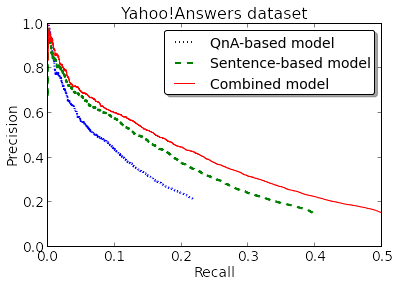
\includegraphics[width=0.99\textwidth]{img/cqarelextract_qa_vs_sent_ya}
    \label{figure:factoid:cqarelextract:pr_curve:ya}
\end{subfigure}
\begin{subfigure}[h]{0.45\textwidth}
    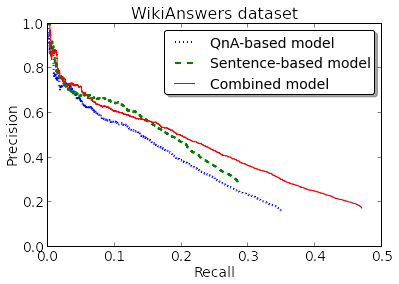
\includegraphics[width=0.99\textwidth]{img/cqarelextract_qa_vs_sent_wa}
    \label{figure:factoid:cqarelextract:pr_curve:wa}
\end{subfigure}
\begin{subfigure}[h]{0.45\textwidth}
    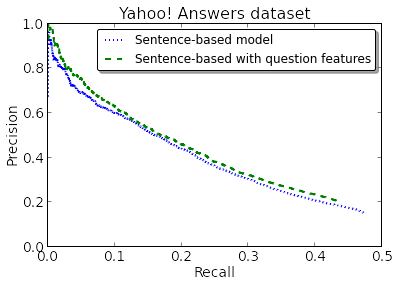
\includegraphics[width=0.99\textwidth]{img/cqarelextract_noqf_vs_qf}
    \label{figure:factoid:cqarelextract:noqf_vs_qf}
\end{subfigure}
\caption{Precision-Recall curves for QnA-based vs sentence-based models and sentence-based model with and without question features.}
\label{figure:factoid:cqarelextract:pr_curve}
\end{figure}

\begin{table}
\centering
\small
\begin{tabular}{p{4.7cm}|ccc|ccc}
& \multicolumn{3}{c|}{Yahoo! Answers} & \multicolumn{3}{c}{WikiAnswers}\\
& QnA & Sent. & Comb. & QnA & Sent. & Comb.\\
\hline
F-1 score & 0.219 & 0.276 & 0.310 & 0.277 & 0.297 & 0.332\\
Number of correct extractions & 3229 & 5900 & 7428 & 2804 & 2288 & 3779 \\
Correct triples not extracted by other model & 20.5\% & 56.5\% & - & 39.4\% & 25.8\% & - \\
\end{tabular}
\caption{Results for relation extraction of QnA-, sentence-based and combined models on Yahoo!~Answers and WikiAnswers datasets.}
\label{table:factoid:cqarelextract:results}
\end{table}

Results demonstrate that from 20.5\% to 39.4\% of correct triples extracted by the QnA-based model are not extracted by the baseline model, and the combination of both models is able to achieve higher precision and recall.
Unfortunately, comparison of the sentence-based model with and without question-based features (Figure~\ref{figure:factoid:cqarelextract:pr_curve}) did not show a significant difference.

\subsection{Analysis and Discussion}
\label{section:factoid:cqarelextract:analysis}

To get an idea of typical problems of the QnA-based model we sampled and manually judged extracted high confidence examples that are not present in Freebase (and thus are considered incorrect for precision-recall analysis).

The major reason (40\%) of false positive extractions is errors in entity linking.
For example: ``\textit{Who is Tim O'Brien? He was born in Austin on October 1, 1946}''.
The model was able to correctly extract [Tim O'Brien, date\_of\_birth, October 1, 1946], however, Tim O'Brien was linked to a wrong person.
In a number of cases (16\%) our discourse model turns out to be too simple and fails for answers, that mention numerous additional information, \eg ``\textit{How old is Madonna really? ...Cher was born on 20 May 1946 which makes her older that Madonna...}''.
A possible solution would be to either restrict QnA-based model to cases when no additional information is present or design a better discourse model with deeper analysis of the answer sentence and its predicates and arguments.
Some mistakes are due to distant supervision errors, for example for the music.composition.composer predicate our model extracts singers as well as composers (which are in many cases the same).

Of course, there are a number of cases, when our extractions are indeed correct but are either missing (33\%) or contradicting with Freebase (8\%).
An example of an extracted fact, that is missing in Freebase is ``\textit{Who is Wole Soyinka? He studied at the University College, Ibadan(1952-1954) and the University of Leeds (1954-1957)}'', and [Wole Soyinka, institution, University of Leeds] is currently not present in Freebase.
Contradictions with Freebase occur because of different precision levels (``pianist'' vs ``jazz pianist'', city vs county, \etc), different calendars used for dates or ``incorrect'' information provided by the user.
An example, when existing and extracted relation instance are different in precision is:``\textit{Who is Edward Van Vleck? Edward Van Vleck was a mathematician born in Middletown, Connecticut}'' we extract [Edward Van Vleck, place\_of\_birth, Middletown], however, the Freebase currently has the USA as his place of birth.

The problem of ``incorrect'' information provided in the answer is very interesting and worth special attention.
It has been studied in CQA research, \eg \cite{shah2010evaluating}, and an example of such QnA pair is: ``\textit{Who is Chandrababu Naidu? Nara Chandra Babu Naidu (born April 20, 1951)}''.
Other authoritative resources on the Web give April 20, 1950, as Chandrababu Naidu's date of birth.
This raises a question of trust to the provided answer and expertise of the answerer.
Many questions on CQA websites belong to the medical domain, \eg people asking advice on different health related topics.
How much can we trust the answers provided to extract them into the knowledge base?
We leave this question to the future work.

Finally, we have seen that only a small fraction of available QnA pairs was annotated with existing Freebase relations, which shows a possible limitation of Freebase schema.
A promising direction for future work is the automatic extraction of new predicates, which users are interested in and which can be useful to answer more future questions.

% \subsection{Summary}
% \label{section:factoid:cqarelextract:summary}

% In this section I described a model for relation extraction from QnA data, which is capable of predicting relations between entities mentioned in question and answer sentences.
% The experiments, conducted on 2 publicly available CQA datasets, showed that our model can extract triples not available to existing sentence-based techniques and can be effectively combined with them for better coverage of a knowledge base population system.

% =-=-=-=-=-=-=-=-=-=-Cqa Relation Extraction: End-=-=-=-=-=-=-=-=-=-=-=-=-=-=-

% =-=-=-=-=-=-=-=-=-=-=-=-=-=-Text2KB: Begin=-=-=-=-=-=-=-=-=-=-=-=-=-=-=-=-=-

\section{Text2KB: Augmenting Knowledge Base Question Answering with External Text Data}
\label{section:factoid:text2kb}

Existing relation extraction tools are not perfect, in particular, due to recall losses a lot of information is left behind.
Moreover, extractions contain a certain level of incorrect information due to precision losses.
Therefore, by applying relation extraction we are lowering the upper bound of the performance of an underlying question answering system.
An alternative approach is to keep the information in its raw unstructured format and design a way to use it along with KB.
In this section, I describe a novel factoid question answering system, that utilizes available textual resources to improve different stages of knowledge base question answering (KBQA).
This work was presented as a full paper at SIGIR 2016 conference~\cite{Savenkov:2016:KBE:2911451.2911536}.

KBQA systems must address three challenges, namely, question entity identification (to anchor the query process); candidate answer generation; and candidate ranking.
We will show that these challenges can be alleviated by the appropriate use of external textual data.
Entity identification seeds the answer search process, and therefore the performance of the whole system greatly depends on this stage~\cite{yao-scratch-qa-naacl2015}.
The question text is often quite short, may contain typos and other problems, that complicate entity linking.
Existing approaches are usually based on dictionaries that contain entity names, aliases and some other phrases, used to refer to the entities \cite{SPITKOVSKY12.266}.
These dictionaries are noisy and incomplete, \eg to answer the question \textit{``what year did tut became king?''} a system needs to detect a mention \textit{``tut''}, which refers to the entity \texttt{Tutankhamun}.
If a dictionary does not contain a mapping \textit{``tut''} $\rightarrow$ \texttt{Tutankhamun}, as happens for one of the state-of-the-art systems, it will not be able to answer the question correctly.
Such less popular name variations are often used along with full names inside text documents, for example, to avoid repetitions.
Therefore, we propose to look into web search results to find variations of question entity names, which can be easier to link to a KB (Figure~\ref{figure:factoid:text2kb:web_search_entitylink}).
This idea has been shown effective in entity linking for web search queries\footnote{\href{url}{http://web-ngram.research.microsoft.com/ERD2014/}} \cite{SMAPH_ERD:2014}.

\begin{figure}[t]
\centering
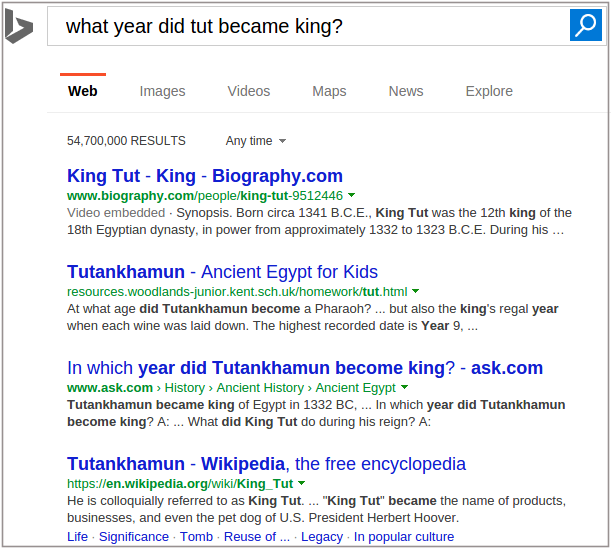
\includegraphics[width=0.75\textwidth]{img/web_search_entitylink}
\caption{Web search results for the question \textit{``what year did tut became king?''}, which mention both the full name of the king and the correct answer to the question.}
\label{figure:factoid:text2kb:web_search_entitylink}
\end{figure}

After question entities have been identified, answer candidates need to be generated and ranked to select the best answer.
A candidate query includes one or multiple triple patterns with predicates, corresponding to words and phrases in the question.
Existing knowledge base question answering approaches~\cite{bastmore:cikm:2015:aquu,BerantCFL13:sempre,BerantL14:parasempre,berant2015imitation,BordesCW14:emnlp,yao2014freebase} rely on a lexicon, learned from manually labeled training data, and supported by additional resources, such as question paraphrases \cite{BerantL14:parasempre} and weakly labeled sentences from a large text collection \cite{YaoD14}.
Such training data tends to be small compared to the number of different predicates in a KB, and therefore the coverage of these lexicons is limited.
By our estimate, in a popular WebQuestions KBQA dataset~\cite{BerantCFL13:sempre}, the answers to $\sim$5.5\% of test questions (112 out of 2032) involve a predicate that does not appear as a ground truth in the training set.
For example, the RDF triple \texttt{[Bigos, food.dish.type\_of\_dish1, Stew]} answers the question \textit{``what are bigos?''}, but no other examples in the training set involve this predicate.
In addition, a lexicon needs to cover all different ways a predicate can be asked about.
For example, questions \textit{``who did jon gosselin cheat with?''} and \textit{``who is the woman that john edwards had an affair with?''} are answered by the same KB predicate but use different language.
Therefore, the presence of the first question in a training set may not help to answer the second question.
On the other hand, traditional Text-QA systems benefit from the redundancy of the information on the Web, where the same facts are stated multiple times in many different ways~\cite{lin2007exploration}.
This increases the chances of a good lexical match between a question and answer statements, which makes even some relatively simple counting-based techniques quite effective~\cite{brill2002analysis}.
The model I developed adapts these ideas from text-based question answering for KBQA.

The general architecture and an example use case of Text2KB is presented on Figure~\ref{figure:factoid:text2kb:model}.
Text2KB is based on the information extraction approach to knowledge base question answering~\cite{YaoD14}, in particular, it extends the Aqqu system of H.Bast et al.~\cite{bastmore:cikm:2015:aquu}, which is one of the best performing open source KBQA system on the WebQuestions dataset.
The left part of the Figure~\ref{figure:factoid:text2kb:model} describes a typical architecture of IE-based KBQA systems, and the right part introduces additional external text data sources, namely Web search results, community question answering (CQA) data, and a collection of documents with detected KB entity mentions.
First, I describe the main stages of the information extraction approach to knowledge base question answering using Aqqu, the baseline system, as an example.

\begin{figure}[t]
\centering
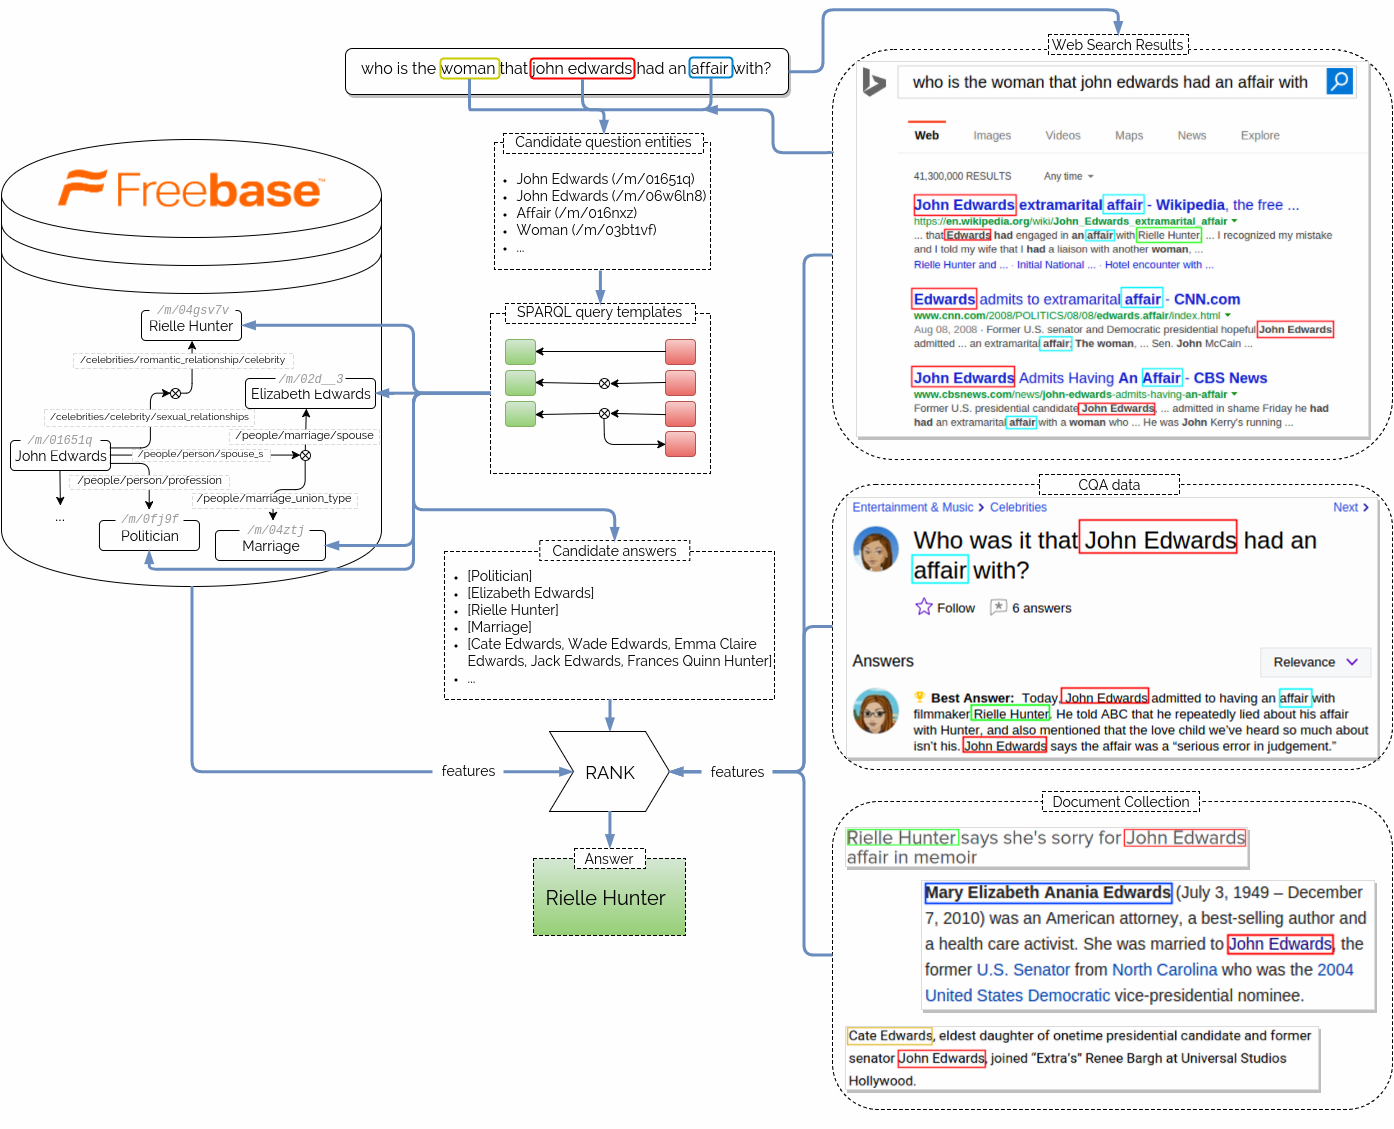
\includegraphics[width=\textwidth]{img/text2kb_model}
\caption{The architecture of the Text2KB Question Answering system.}
\label{figure:factoid:text2kb:model}
\end{figure}

\subsection{Baseline Approach}
\label{section:factoid:text2kb:baseline}

The first stage of the knowledge base question answering process is the identification of question topic entities, which are used as sources for the answer search process.
For concreteness, consider a question from the WebQuestions dataset \textit{``who is the woman that john edwards had an affair with?''}.
Here, the entity \texttt{John Edwards} with Freebase id \texttt{/m/01651q} is the main question entity.
However, Freebase contains millions of entities and it can be difficult to identify the topical ones (\eg entities \texttt{Woman} and \texttt{Affair} are also present in Freebase), or to disambiguate and choose between \texttt{John Edwards} a politician (\texttt{/m/01641q}), an American racing driver (\texttt{/m/06zs089}) and other people with the same name.
Aqqu considers all spans of question words under certain conditions on part of speech tags and uses an entity names lexicon \cite{SPITKOVSKY12.266} to map phrases to potential entities.
Most reported systems, including Aqqu, do not disambiguate entities at this stage, but rather keep a set of candidates along with some information about their popularities (\eg number of mentions in the collection), and mention scores $p(entity| mention\ text)$.

At the next stage, SPARQL query candidates are generated by exploring the neighborhood of the question topic entities using a predefined set of query templates.
Each query template has question entities, predicates and answer placeholders.
The majority of the answers in the WebQuestions dataset can be covered by just 3 templates (q\_entity - question entity, a\_entity - answer entity, cvt\_node - Freebase mediator node, which represents tuples with more than 2 arguments):
\\

\begin{minipage}{\linewidth}
\begin{lstlisting}[frame=single,basicstyle=\small]
SELECT DISTINCT ?a_entity {
   <q_entity> <predicate> ?a_entity .
}
\end{lstlisting}
\end{minipage}

\begin{minipage}{\linewidth}
\begin{lstlisting}[frame=single,basicstyle=\small]
SELECT DISTINCT ?a_entity {
   <q_entity> <predicate_1> ?cvt_node .
   ?cvt_node <predicate_2> ?a_entity .
}
\end{lstlisting}
\end{minipage}

\begin{minipage}{\linewidth}
\begin{lstlisting}[frame=single,basicstyle=\small]
SELECT DISTINCT ?a_entity {
   <q_entity_1> <predicate_1> ?cvt_node .
   ?cvt_node <predicate_2> <q_entity_2> .
   ?cvt_node <predicate_3> ?a_entity .
}
\end{lstlisting}
\end{minipage}

The first template retrieves a set of entities that are directly connected to the given question entity via a certain predicate.
The second template accounts for the presence of a mediator node, that groups together arguments of a multi-argument relation.
And the last template looks for cases when a question also mentions another argument of a multi-argument relation, \eg \texttt{Captain Kirk} and \texttt{Star Trek} for the question \textit{``who played captain kirk in star trek movie?''}.

Each query candidate is represented with a set of features, that includes the scores for linked question entities, various scores for matching between question term n-grams and query predicates, the size of the results list, \etc
The final stage of the question answering process is filtering and ranking.
The Aqqu system employs a pairwise learning-to-rank model, trained on part of the dataset.
For each pair of candidate answers, Aqqu creates an instance, which contains 3 groups of features: features of the first, the second candidate in the pair and the differences between the corresponding features of the candidates. Specifically, a Random Forest model is used in the provided Aqqu implementation. 
A pair where the first candidate is better than the second belongs to class +1, and -1 otherwise.
To reduce the number of pairs for the final ranking, Aqqu includes a simplified linear filtering model, which is trained to detect incorrect answers with high precision. 

In Text2KB we also introduced a couple of extensions to the original Aqqu system, which does not involve external text data.
We noticed that since Aqqu does not use information about the answer entity Freebase types, in many cases it returns an answer that is incompatible with the question: \eg state instead of county \etc
Therefore, we trained a model to return a score that measures compatibility between the question and answer entities, based on the entity notable types and question uni- and bi-grams as features, similar to Aqqu's relations score model.
A second extension introduced a new date range query template, which helps solve cases like \textit{``what team did david beckham play for in 2011?''}, where we need to look at the ranges of dates to determine whether an answer candidate satisfies the question.
\\

\begin{minipage}{\linewidth}
\begin{lstlisting}[frame=single,basicstyle=\small]
SELECT DISTINCT ?a_entity {
   <q_entity_1> <predicate_1> ?cvt_node .
   ?cvt_node <from_predicate> ?date_from .
   ?cvt_node <to_predicate> ?date_to .
   ?cvt_node <predicate_2> ?a_entity .
   FILTER ( <question_date> >= ?date_from AND
            <question_date> <= ?date_to )
}
\end{lstlisting}
\end{minipage}


\subsection{Text2KB Model}
\label{section:factoid:text2kb:model}

Text2KB improves the baseline knowledge base question answering model by utilizing textual resources on various stages of the pipeline.
Our model uses web search results to improve question analysis, \ie identify question topic, and extract additional features to support generated answer candidates.
Question-answer pairs from CQA archives are used to learn associations between question words and KB predicates, and score candidate SPARQL queries.
Finally, a text collection annotated with KB entity mentions is used to build a language model for entity pairs, and generate answer ranking features.

\textbf{Web search results for question understanding and answer ranking.}
Traditional TextQA systems rely on search results to retrieve relevant documents, which are then used to extract answers to users' questions.
Relevant search results mention question entities multiple times and in various forms, which can be helpful for entity linking \cite{SMAPH_ERD:2014}.
Furthermore, retrieved document set often contains multiple occurrences of the answer, which can be a strong signal for candidate ranking~\cite{lin2007exploration}.

To obtain related web search results, Text2KB issues the question as a query to a search engine\footnote{In our experiments, we use the Bing Web Search API \href{url}{https://www.microsoft.com/cognitive-services/en-us/bing-web-search-api} and local Wikipedia search using Lucene}, extracts top 10 result snippets and the corresponding documents.
Next, Text2KB uses Aqqu entity linking module to detect KB entity mentions in both snippets and documents.

Question text provides only a limited context for entity disambiguation and linking; additionally, the entity name can be misspelled or an uncommon variation used.
This complicates the task of entity identification, which is the foundation of KB question answering process.
Fortunately, web search results help with these problems, as they usually contain multiple mentions of the same entities and provide more context for disambiguation.
Text2KB uses the search result snippets to \textit{expand} the set of detected question entities.
More specifically, we count the frequencies of each entity mentioned in search snippets, and most popular ones with names similar to some of the question terms are added to the list of topical entities.
The goal of this similarity condition is to keep only entities that are likely mentioned in the question text and filter out related, but different entities.
To estimate the similarity between a name and question tokens, we use Jaro-Winkler string distance.
An entity is added to the list of question entities if at least one of its tokens $e_t$ has high similarity with one of the question tokens $q_t$ excluding stopwords ($Stop$):
$$max_{e_t \in M \backslash Stop, q_t \in Q \backslash Stop} 1 - dist(e_t, q_t) \geq 0.8$$

The information stored in KBs can also be present in other formats, \eg text statements.
For example, on Figure \ref{figure:factoid:text2kb:web_search_entitylink} multiple search snippets mention the date when Tutankhamun became a king.
TextQA systems use such passages to extract answer to users' questions.
However, text may not provide sufficient context information about the mentioned entities, and systems have to infer the useful details, \eg entity types, which can be problematic \cite{yih2014semantic}.
On the other hand, KBQA systems can utilize all the available KB knowledge about the entities in a candidate answer and would benefit from additional text-based information to improve ranking.
More specifically, Text2KB proceeds as follows (full list of features is given in Table~\ref{table:factoid:text2kb:features}):

\begin{enumerate}
\item Precompute term and entity IDFs. We used Google n-grams corpus to approximate terms IDF by collection frequencies and available ClueWeb Freebase entity annotations\footnote{\href{url}{http://lemurproject.org/clueweb09/FACC1/}} to compute entity IDF scores.
\item Each snippet $s_i$ and document $d_i$ are represented by two TF-IDF vectors of lowercased tokens ($t_{s_i}$ and $t_{d_i}$) and mentioned entities ($e_{s_i}$ and $e_{d_i}$).
\item In addition, vectors of all snippets and all documents are merged together to form combined token and entity vectors: $t_{\cup s_i}$, $t_{\cup d_i}$, $e_{\cup s_i}$ and $e_{\cup d_i}$.
\item Each answer candidate $a_j$ is also represented as TF-IDF vector of terms (from entity names), and entities: $t_{a_j}$ and $e_{a_j}$
\item Cosine similarities between answer and each of 10 snippet and document vectors are computed: $\cos(t_{s_i}, t_{a_j})$, $\cos(t_{d_i}, t_{a_j})$ and $\cos(e_{s_i}, e_{a_j})$, $\cos(e_{d_i}, e_{a_j})$.
We use the average score and the maximum score as features.
\item We also compute answer similarities with the combined snippet and document vectors: $\cos(t_{\cup s_i}, t_{a_j})$, $\cos(e_{\cup s_i}, e_{a_j})$, $\cos(t_{\cup d_i}, t_{a_j})$, $\cos(e_{\cup d_i}, e_{a_j})$.
\end{enumerate}

\textbf{CQA data for matching questions to predicates.}
Recall that a major challenge in KBQA is that natural language questions do not easily map to entities and predicates in a KB.
An established approach for this task is supervised machine learning, which requires labeled examples of questions and the corresponding answers to learn this mapping, which can be expensive to construct.
Researchers have proposed to use weakly supervised methods to extend a lexicon with mappings learned from \textit{single sentence statements} mentioning entity pairs in a large corpus \cite{YaoD14}.
However, the language used in questions to query about a certain predicate may differ from the language used in statements.
In Section~\ref{section:factoid:cqarelextract} we demonstrated how distant supervision can be applied to question-answer pairs from CQA archives for a related task of information extraction for knowledge base completion.
In a similar way, we use weakly labeled collection of question-answer pairs to compute {\em associations} between question terms and predicates to \textit{extend} system's lexicon (Figure~\ref{figure:factoid:text2kb:cqa_example}).
We emphasize that this data does not replace the mappings learned from single sentence statements, which are already used by our baseline system, but rather introduces the new ones learned from the CQA data.

\begin{figure}[t]
\centering
\fbox{
 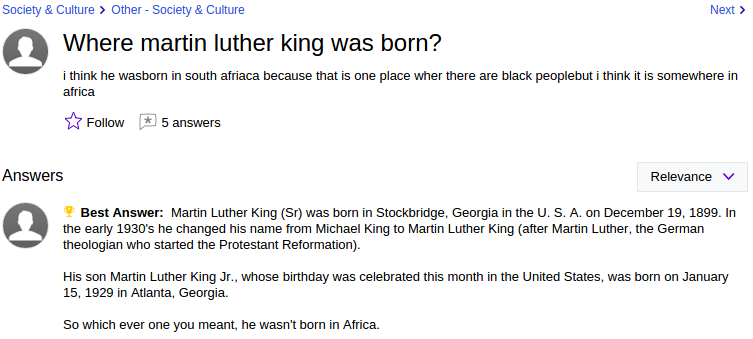
\includegraphics[width=0.7\textwidth]{img/cqa_example}
}
\caption{Example of a question and answer pair from Yahoo! Answers CQA website.}
\label{figure:factoid:text2kb:cqa_example}
\end{figure}

For our experiments, we use 4.4M questions from Yahoo! WebScope L6 dataset\footnote{\href{url}{https://webscope.sandbox.yahoo.com/}}.
Question and answer texts were run through an entity linker, that detected mentions of Freebase entities.
Next, we use distant supervision assumption to label each question-answer pair with predicates between entities mentioned in the question and in the answer.
These labels are used to learn associations between question terms and predicates by computing pointwise mutual information scores (PMI) for each term-predicate pair.
Examples of scores for some terms are given in Table~\ref{table:factoid:text2kb:cqa_npmi}.

\begin{table}[t]
\centering
\begin{tabular}{rp{8.5cm}l}
Term & Predicate & PMI\\
\hline
born & \texttt{people.person.date\_of\_birth} & 3.67\\
 & \texttt{people.person.date\_of\_death} & 2.73\\
 & \texttt{location.location.people\_born\_here} & 1.60\\
\hline
kill & \texttt{people.deceased\_person.cause\_of\_death} & 1.70\\
& \texttt{book.book.characters} & 1.55\\
\hline
currency & \texttt{location.country.currency\_formerly\_used} & 5.55 \\
& \texttt{location.country.currency\_used} & 3.54 \\
\hline
school & \texttt{education.school.school\_district} & 4.14 \\
& \texttt{people.education.institution} & 1.70\\
& \texttt{sports.school\_sports\_team.school} & 1.69 \\
\hline
illness & \texttt{medicine.symptom.symptom\_of} & 2.11\\
& \texttt{medicine.decease.causes} & 1.68\\
& \texttt{medicine.disease.treatments} & 1.59\\
\hline
win & \texttt{sports.sports\_team.championships} & 4.11\\
& \texttt{sports.sports\_league.championship} & 3.79\\
\end{tabular}
\caption{Examples of term-predicate pairs with high PMI scores, computed using distant supervision from a CQA collection.}
\label{table:factoid:text2kb:cqa_npmi}
\end{table}

In Text2KB we evaluate candidate answer predicates by using the association (\eg PMI) scores between predicates and the question terms (missing pairs are given a score of 0).
The minimum, average and maximum of these values are used as features to represent a candidate answer.
Such associations data can be sparse, we also use pretrained word2vec word embeddings\footnote{\href{url}{https://code.google.com/p/word2vec/}}.
We compute predicate embeddings by taking a weighted average of term vectors from predicate's PMI table.
Each term vector is weighted by its PMI value (terms with a negative score are skipped).
Then, we compute cosine similarities between predicate vector and each of the question term vectors and take their minimum, average, maximum as features.
Finally, we average embeddings of question terms and compute its cosine similarity with the predicate vector (full list of features is given in Table~\ref{table:factoid:text2kb:features}).

\textbf{Estimating entity associations using a semantically annotated text collection.}
A key step for ranking candidate answers is to estimate whether the question and answer entities are related in a way asked in the question.
Existing KBQA approaches usually focus on scoring the mappings between question phrases and KB concepts from a candidate SPARQL query.
However, textual data can provide another angle on the problem, as question and answer entities are likely to be mentioned together somewhere in text passages.
For example, in the bottom right corner of Figure~\ref{figure:factoid:text2kb:model} we can see some passages that mention a pair of people, and the context of these mentions explains the nature of the relationships.
This data can be viewed as additional edges in a KB, which connect pairs of entities and have associated language models, estimated from text phrases, that mention these entities.
Such edges do not have to coincide with the existing KB edges and can connect arbitrary pairs of entities, that are mentioned together in the text, therefore extend the KB.

We use the ClueWeb12 corpus with existing Freebase entity annotations and count different terms that occur in the context of a mention of a pair of different entities (we only consider mentions within 200 characters of each other).
To compute this unigram language model we use the terms separating the entities, as well as the terms within a small window (\eg 100 characters) before and after the entity mentions.
A small sample of this data is presented in Table~\ref{table:factoid:text2kb:clueweb_entitypairs_langmodel}.

\begin{table}
\centering
\small
\begin{tabular}{rlp{7cm}}
Entity 1 & Entity 2 & Frequent terms\\
\hline
 & Rielle Hunter & campaign, affair, mistress, child, former ...\\
 & Cate Edwards & daughter, former, senator, courthouse, greensboro, eldest ...\\
John Edwards & Elizabeth Edwards & wife, hunter, campaign, affair, cancer, rielle, husband ...\\
 & Frances Quinn & daughter, john, rielle, father, child, former, paternity...\\
 \hline
\end{tabular}
\caption{Example of entity pairs along with the most popular terms mentioned around the entities in ClueWeb12 collection.}
\label{table:factoid:text2kb:clueweb_entitypairs_langmodel}
\end{table}

We use this data to compute candidate ranking features as follows.
Consider question words $Q$ and an answer candidate, which contains a question entity $e_1$ and one or more answer entities $e_2$.
For each answer candidate, we compute a language model score:
$$p(Q|e_1, e_2) = \prod_{t\in Q} p(t | e_1, e_2)$$
and use the minimum, average and maximum over all answer entities as features.
To address the sparsity problem, we again use embeddings, 
\ie for each entity pair a weighted (by counts) average embedding vector of terms is computed and minimum, average and maximum cosine similarities between these vectors and question token embeddings are used as features (full list of features is given in Table~\ref{table:factoid:text2kb:features}).

\textbf{Internal text data to enrich entity representation.}
In addition to external text data, many knowledge bases, including Freebase, contain text data as well, \eg Freebase includes a description paragraph from Wikipedia for many of its entities.
These text fragments provide a general description of entities, which may include information relevant to the question \cite{Sun:2015:ODQ:2736277.2741651}.
For completeness, we include them in our system as well.
Each entity description is represented by a vector of tokens, and a vector of mentioned entities.
We compute cosine similarities between token and entity vectors of the question and description of each of the answers and use the minimum, average and maximum of the scores as features.

The final list of text-based features used in Text2KB model is presented in Table~\ref{table:factoid:text2kb:features}.

\begin{table}[h!]
\centering
\small
\begin{tabular}{r|p{8cm}}
Data Source & Feature\\
\hline
Search results (\texttt{Wiki} or \texttt{Web}) & - number of entity mentions in search results \\
 & - max and average tf-idf cosine similarity between answer and search snippets/documents \\
 & - max and average embeddings cosine similarity between question tokens and search snippets/documents \\
CQA data (\texttt{CQA}) & - sum, average, minimum and maximum PMI scores between question tokens and answer predicates \\
 & - sum, average, minimum and maximum embeddings cosine similarity scores between question tokens and PMI-weighted answer predicates tokens \\
Text collection (\texttt{CL}) & - min, max and average entity-pair language model score for question topic and answer entities \\
 & - min, max and average entity-pair embeddings score for question topic and answer entities \\
\end{tabular}
\caption{The list of text-based features used in the Text2KB model.}
\label{table:factoid:text2kb:features}
\end{table}

\subsection{Experimental Results}
\label{section:factoid:text2kb:eval}

This section reports the experimental setup, including the dataset and metrics, as well as the main methods compared for evaluating the performance of our Text2KB system. Additionally, we describe a series of ablation studies to analyze the contribution of different system components.

\textbf{Methods Compared}.
We compare our system, Text2KB, to state-of-the-art approaches, notably:
\begin{itemize}[noitemsep]
\item{\textbf{Aqqu}}: a state-of-the-art baseline KBQA system~\cite{bastmore:cikm:2015:aquu}, described in Section~\ref{section:factoid:text2kb:baseline}.
\item{\textbf{Text2KB(Web search)}}: Our Text2KB system, using the Bing search engine API over the Web. 
\item{\textbf{Text2KB(Wikipedia search)}}: Our Text2KB system, using the standard Lucene search engine over the February 2016 snapshot of the English Wikipedia, in order to validate our system without the potential ``black-box'' effects of relying on a commercial Web search engine (Bing) and changing corpus (Web).
\item{\textbf{STAGG}}: One of the best\footnote{It was the best result published before summer 2016, \ie the camera-ready version of my paper, describing Text2KB system.} current KBQA systems~\cite{yih:ACL:2015:STAGG} as measured on the WebQuestions dataset.
\end{itemize}
Additionally, other previously published results on WebQuestions are included to provide context for the improvements introduced by our Text2KB system.

\textbf{Datasets}.
I followed the standard evaluation procedure for the WebQuestions dataset and used the original 70-30\% train-test split (3,778 training and 2,032 test instances). Within the training split, 10\% was set aside for validation to tune the model parameters and only the best-performing set of parameters selected on the validation data was used to report the results on the official test split.

\textbf{Evaluation Metrics}. 
Recent papers using the WebQuestions dataset have primarily used the average F1-score as the main evaluation metric, defined as:
$avg\ F1 = \frac{1}{|Q|} \sum_{q \in Q} f1(a^*_q, a_q)$
$$f1(a^*_q, a_q) = 2\frac{precision(a^*_q,a_q) recall(a^*_q,a_q)}{precision(a^*_q,a_q) + recall(a^*_q,a_q)}$$
$precision(a^*_q, a_q)=\frac{|a^*_q \cap a_q|}{|a_q|}$ and $recall(a^*_q, a_q) = \frac{|a^*_q \cap a_q|}{|a^*_q|}$, $a^*_q$ and $a_q$ are correct and given answers to the question q, which can be lists of entities.
Additionally, I report average precision and recall, to gain a better understanding of the trade-offs achieved by different methods.

\begin{table}[t]
\centering
\small
\begin{tabular}{rp{1.9cm}p{1.7cm}p{1.9cm}p{1.2cm} }
System & $\overline{Recall}$ & $\overline{Precision}$ & F1 of $\overline{P}$ \& $\overline{R}$ & $\overline{F1}$ \\
\hline
OpenQA \cite{Fader:2014:OQA:2623330.2623677} & - & - & - & 0.35 \\
YodaQA \cite{baudivs2015yodaqa} & - & - & - & 0.343 \\
\hline
Jacana \cite{YaoD14} & 0.458 & 0.517 & 0.486 & 0.330\\
SemPre \cite{BerantCFL13:sempre} & 0.413 & 0.480 & 0.444 & 0.357\\
Subgraph Embed \cite{BordesCW14:emnlp} & - & - & 0.432 & 0.392\\
ParaSemPre \cite{BerantL14:parasempre} & 0.466 & 0.405 & 0.433 & 0.399\\
Kitt AI \cite{yao-scratch-qa-naacl2015} & 0.545 & 0.526 & 0.535 & 0.443\\
AgendaIL \cite{berant2015imitation} & 0.557 & 0.505 & 0.530 & 0.497\\
DepLambda \cite{reddy2016transforming} & 0.611 & 0.490 & 0.544 & 0.503 \\
STAGG \cite{yih2014semantic} & 0.607 & 0.528 & 0.565 & 0.525\\
Textual Evidence\cite{xu2016enhancing} & - & - & - & 0.533 \\
FMN \cite{jain2016question} & \textbf{0.649} & \textbf{0.552} & \textbf{0.597} & \textbf{0.557}\\
\hline
Aqqu (baseline) \cite{bastmore:cikm:2015:aquu} & 0.604 & 0.498 & 0.546 & 0.494\\
Text2KB$_{Wiki Search}$ & \textbf{0.632}$_{(+4.6\%)}^*$  & 0.498 & 0.557$_{(+2.0\%)}^*$ & 0.514$_{(+4.0\%)}^*$ \\
Text2KB$_{Web Search}$ & \textbf{0.635}$_{(+5.1\%)}^*$ & 0.506$_{(+1.6\%)}^*$ & \textbf{0.563}$_{(+3.1\%)}^*$ & \textbf{0.522}$_{(+5.7\%)}^*$ \\
\end{tabular}
\caption{Average performance metrics of the Text2KB system on WebQuestions dataset compared to the existing approaches. The differences of scores marked * from the baseline Aqqu system are significant with p-value $<$ 0.01.}
\label{table:factoid:text2kb:webquestions_results}
\end{table}

\textbf{Main Results.}
The results of existing approaches and our Text2KB system are presented in Table~\ref{table:factoid:text2kb:webquestions_results}.
We should note, that text-based QA systems typically return a ranked list of answers, whereas many answers on WebQuestions dataset are lists, which complicates the comparison between KBQA and text-based systems.
The result reported for YodaQA system is the F1 score at position 1.
As we can see, Text2KB significantly improves over the baseline system.

\textbf{Data Source and Features Contribution}.
To analyze the contribution of the features and data sources I introduced, I report results from a series of ablation studies. For convenience, I introduce the following short-hand notations for different components of our system:

\begin{itemize}[noitemsep]
\item \texttt{T} - notable type score model as a ranking feature
\item \texttt{DF} - date range filter-based query template
% \item TF - using notable type based filter
\item \texttt{WebEnt} - using web search result snippets for question entity identification
\item \texttt{WikiEnt} - using wikipedia search result snippets for question entity identification
\item \texttt{Web} - using web search results for feature generation
\item \texttt{Wiki} - using wikipedia search results for feature generation
\item \texttt{CQA} - using CQA-based \texttt{[question term, KB predicate]} PMI scores for feature generation
\item \texttt{CW} - features, computed from entity pairs language model, estimated on ClueWeb
\end{itemize}

In the results table I will use the notation \texttt{+$<$comp$>$} for a system with a certain component added, and \texttt{-$<$comp$>$} when it is removed.
For example, the baseline system will be denoted as ``\texttt{Aqqu}''.
The same system with additional date range filter query templates and notable types score model is denoted as ``\texttt{Aqqu +DF+T}'', which represents the same system as ``\texttt{Text2KB -WebEnt-Web-CQA-CL}'' (we will call it Text2KB (base)).
Our full system ``\texttt{Text2KB}'' can be also denoted as ``\texttt{Aqqu +DF+T+WebEnt+Web+CQA+CL}''.

First, I analyze the improvements introduced by different components of the system (Table~\ref{table:factoid:text2kb:ablation:entities_vs_features}).
As we can see, additional date range filters and notable types model (\texttt{Aqqu+DF+T}) are responsible for an increased recall and a drop in precision compared to the baseline model.
Features generated from Wikipedia search results, CQA data and ClueWeb entity pair language models (\texttt{+Wiki+CQA+CL}) improve average F1 by 0.007 (+1.4\%) compared to the base model, adding entity linking using Wikipedia search results improves results even more (+3\%).

Web search results (\texttt{+Web+CQA+CL}) turned out to be more helpful than Wikipedia results (\texttt{+Wiki+CQA+CL}), which is natural since Wikipedia is a subset of the web.
This was one of the reasons we did not combine Wikipedia and Web search together.
Finally, entity linking and all text-based features combined achieves an even higher score, proving that their contributions are independent.

I now analyze the contribution of the different data sources.
I will remove a group of web search, CQA or Clueweb-based features and see how the performance of the whole system changes (Table~\ref{table:factoid:text2kb:ablation:features}).
As we can see, all data sources have an impact on the system performance, and web search results based features provide the most useful signal for answer ranking.

Figure~\ref{figure:factoid:text2kb:ablation:feature_importances} plots a subset of features ranked by their Gini index-based importance scores.
The figure supports the observation that web search results features are the most useful, however, other text data sources also contribute to the improvement.

\begin{table}
\centering
\begin{tabular}{rlll}
System & Recall & Prec & F1 \\
\hline
\texttt{Aqqu} & 0.604 & 0.498 & 0.494\\
\texttt{Text2KB (base) = Aqqu+DF+T} & 0.617 & 0.481 & 0.499 \\
\hline
\texttt{+Wiki+CQA+CL} & 0.623 & 0.487 & 0.506 \\
\texttt{+WikiEnt +Wiki+CQA+CL} & 0.632 & 0.498 & 0.514 \\
\hline
\texttt{+WebEnt} & 0.627 & 0.492 & 0.508 \\
\texttt{+Web+CQA+CL} & 0.634 & 0.497 & 0.514 \\
\texttt{+WebEnt +Web+CQA+CL} & 0.635 & 0.506 & 0.522 \\
\end{tabular}
\caption{Average Recall, Precision (Prec), and F1 of Aqqu and Text2KB system with and without different components. +A means that a component A is added to the Text2KB (base) system.}
\label{table:factoid:text2kb:ablation:entities_vs_features}
\end{table}

\begin{table}[h]
\centering
\begin{tabular}{rlll}
System & Recall & Prec &  F1 \\
\hline
\texttt{Text2KB} (Web search) & 0.635 & 0.506 & 0.522 \\
\hline
% THIS PART ANSWERS HOW GOOD ARE EACH OF THE PROPOSED DATASETS
% extent_cqa_clueweb_dates_typemodel_rf100.log : -web
\texttt{Text2KB -Web} & 0.633 & 0.496 & 0.513 \\
% extent_web_clueweb_dates_typemodel_rf100.log : -cqa
\texttt{Text2KB -CQA} & 0.642 & 0.499 & 0.519 \\
% extent_web_cqa_dates_typemodel_rf100.log : -clueweb
\texttt{Text2KB -CL} & 0.644 & 0.505 & 0.523 \\
\hline
% extent_web_dates_typemodel_rf100.log : -clueweb-cqa
\texttt{Text2KB -CQA-CL} & 0.642 & 0.503 & 0.522 \\
% extent_clue_dates_typemodel_rf100.log : -web-cqa
\texttt{Text2KB -Web-CQA} & 0.631 & 0.498 & 0.514 \\
% extent_cqa_dates_typemodel_rf100.log : -web-clueweb
\texttt{Text2KB -Web-CL} & 0.622 & 0.493 & 0.508 \\
%\hline
% extent_web_cqa_clueweb_dates_types_typemodel_rf100.log : everything, including type filters
%\texttt{Text2KB} & 0.6354 & 0.5059 & 0.5223 \\
\end{tabular}
\caption{Average Recall, Precision (Prec), and F1 of Text2KB with and without features based on web search results, CQA data and ClueWeb collection.}
\label{table:factoid:text2kb:ablation:features}
\end{table}

\begin{figure*}
\centering
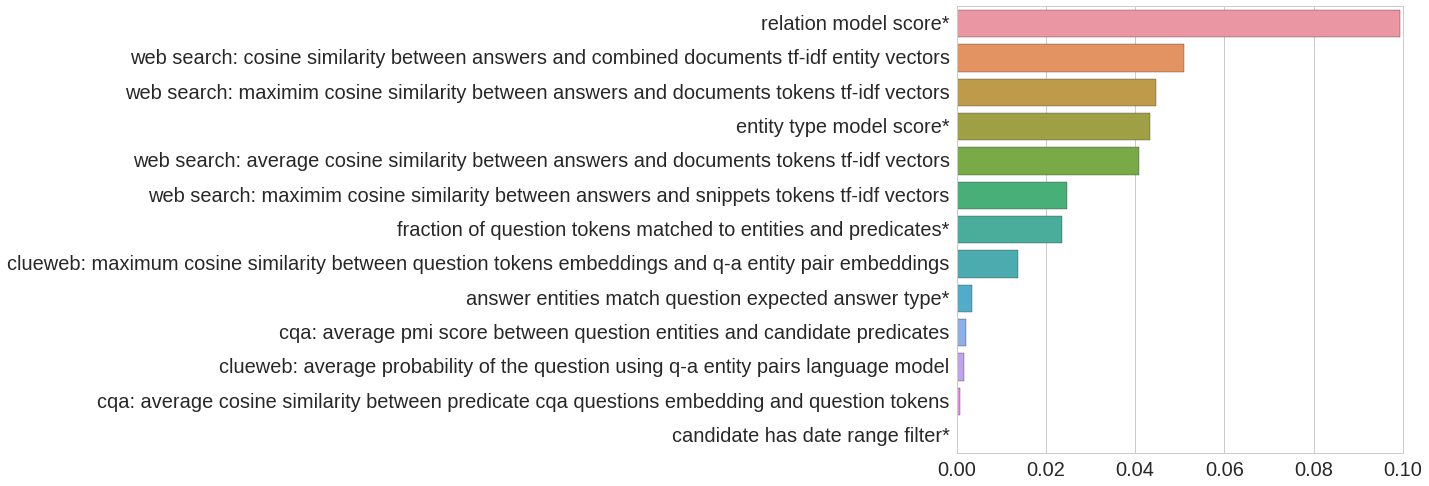
\includegraphics[width=\textwidth]{img/feature_importances}
\caption{A plot of Gini importances of different features of our answer ranking random forest model (features marked * are not text-based and are provided for comparison).}
\label{figure:factoid:text2kb:ablation:feature_importances}
\end{figure*}

In summary, Text2KB significantly outperforms the baseline system, and each of the introduced components contributes to this improvement.
Web search results data turned out to be the most useful resource, and it significantly improves the quality by helping with question entity identification and candidate ranking.
Next, I analyze the system performance in more detail and investigate factors for future extension.

\subsection{Analysis}
\label{section:factoid:approaches:text2kb:analysis}

I now investigate how Text2KB compares to other systems on the same benchmark; then, I investigate in depth the different error modes, which helps identify the areas of most substantial future improvements.

I took an existing KBQA system and demonstrated that by combining evidence from a knowledge base and external text resources we can boost the performance.
A reasonable question is whether the same approach will be helpful for other systems, \eg the best system at the moment of our paper publication -- STAGG~\cite{yih:ACL:2015:STAGG}.
STAGG differs from the baseline system Aqqu in the components: entity linking algorithm, a set of query templates and ranking methods.
Therefore, my approach is ``orthogonal'' to these improvements and should be helpful for STAGG as well.
To support this claim, I made an experiment to combine answers of STAGG and Text2KB.
One of the advantages of the former is its set of filters, that restricts list results to entities of certain type, gender, \etc
Therefore, I combined answers of STAGG and Text2KB using a simple heuristic: I chose to use the answer returned by STAGG if the number of answer entities is less than in the Text2KB answer, otherwise, I used the answer of Text2KB.
Table~\ref{table:factoid:text2kb:combine_stagg} gives the results of the experiment, and as we can see the combination achieves a slightly better average F1 score.
Alternatively, we can look at the Oracle combination of the systems, which always selects the answer with the higher F1.
As we can see such a combination results in a performance of 0.606, which is much higher than either of the systems.

\begin{table}
\centering
\begin{tabular}{rl}
System  & avg F1 \\
\hline
Text2KB & 0.522\\
STAGG~\cite{yih:ACL:2015:STAGG} & 0.525\\
Text2KB + STAGG & 0.532 (+1.3 \%) \\
Text2KB + STAGG (Oracle) & 0.606 (+15.4 \%) \\
\end{tabular}
\caption{Average F1 for combinations of Text2KB and STAGG using a simple heuristic based on the length of the answer list and Oracle upper bound.}
\label{table:factoid:text2kb:combine_stagg}
\end{table}

As I mentioned earlier, answers to 112 of the test questions in the WebQuestions dataset involve predicates that were not observed in the training set, which may be a problem for approaches that rely on a trained lexicon.
I evaluated both systems on these questions, and indeed the performance is very low, \ie the average F1 score of Text2KB is 0.1640 compared to 0.1199 for STAGG\footnote{Unfortunately, the number of questions is too low to show statistical significance (p-value=0.16) of the difference.}.

\begin{figure}
\centering
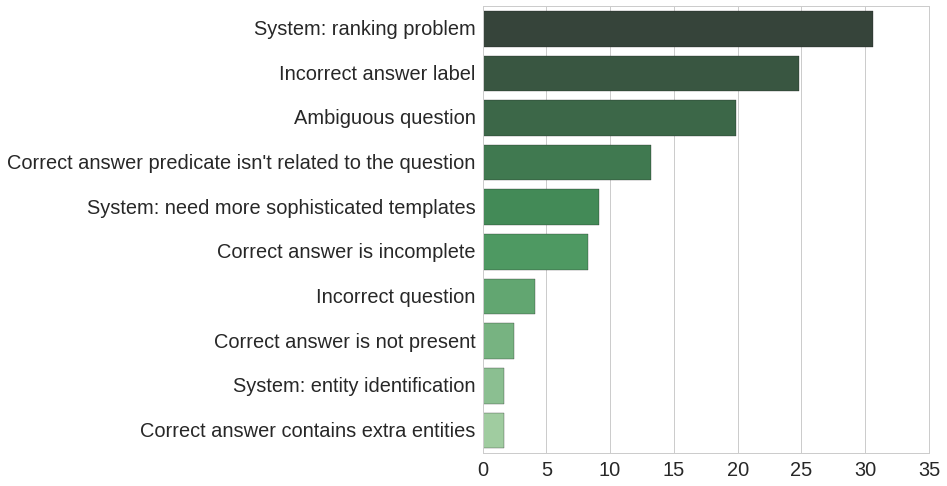
\includegraphics[width=0.7\textwidth]{img/error_analysis}
\caption{Distribution of problems with questions, where Text2KB returns an answer with F1$<$1.}
\label{figure:factoid:text2kb:error_analysis}
\end{figure}

To get better insights into the problems that remain, I collected 1219 questions for which Text2KB did not return a completely correct answer, \ie F1 score $<$ 1.
I manually looked through a couple of hundreds of these examples and grouped the problems into several clusters (Figure~\ref{figure:factoid:text2kb:error_analysis}).

As we can see candidate ranking is still the major problem, and it accounts for $\sim31\%$ of the cases.
The second problem is incorrect ground truth labels (almost 25\% of reported errors).
Another set of questions has incomplete or overcomplete ground truth answer list.
Typical examples are questions asking for a list of movies, books, landmarks, \etc
The ground truth answer usually contains $\sim10$ entities, whereas the full list is often much larger.
This seems to be an artifact of the labeling process, where the answer was selected from the Freebase entity profile page, which shows only a sample of 10 entities, while the rest are hidden behind the ``N values total'' link.
About 20\% of the questions are ambiguous, \ie questions have no strict 1-1 correspondence with any of the predicates and can be answered by multiple ones without any obvious preferences.
For example, the question \textit{``what did hayes do?''} can be answered by profession, occupied position or some other achievements.
Another problem is when there is no predicate that answers the question.
For example, the question \textit{``what do people in france like to do for fun?''} does not have a good match among the facts stored in Freebase.
The ground truth entity \texttt{Cycling} comes from the list Olympic sport competitions country participated\footnote{\texttt{olympics.olympic\_participating\_country.athletes}}.

Text2KB components were quite effective in resolving some of the problems.
Web search results helped identify the right question topical entity in a number of cases, \eg \textit{``what did romo do?''} mentions only the last name of the Dallas Cowboys quarterback and the baseline system were unable to map it to the right entity.
Web search results provides more than enough evidence that ``\textit{romo}'' refers to \texttt{Tony Romo}.
However, there is a number of loses, introduced by added unrelated entities.
For example, the entity \texttt{I Love Lucy} was added for the question \textit{``what was lucille ball?''}, because the term \textit{lucy} had high similarity with \textit{lucille}.
A portion of these problems can be fixed by a better entity linking strategy, \eg \cite{SMAPH_ERD:2014}.
An interesting example, when external text resources improved the performance is the question \textit{``what ship did darwin sail around the world?''}.
This is actually a hard question because the ship entity is connected to the \texttt{Charles Darwin} entity through the ``knownFor'' predicate along with some other entities like \texttt{Natural selection}.
% \footnote{\texttt{user.lindenb.default\_domain.scientist.known\_for}
Thus, the predicate itself is not related to the question, but nevertheless, the name of the ship \texttt{HMS Beagle} is mentioned multiple times in the web search results, and entity pair model computed from ClueWeb also has high scores for the terms ``ship'' and ``world''.

There are several major reasons for the loses, introduced by features based on external text resources.
Some entities often mentioned together and therefore one of them gets high values of co-occurrence features.
For example, the baseline system answered the question \textit{``when did tony romo got drafted?''} correctly, but since \texttt{Tony Romo} is often followed by \texttt{Dallas Cowboys}, Text2KB ranked the team name higher.
Another common problem with our features is an artifact of entity linking, which works better for names and often skips abstract entities, like professions.
For example, the correct answer to the question \textit{``what did jesse owens won?''} is an entity with the name \texttt{Associated Press Male Athlete of the Year}, which is rarely mentioned or it is hard to find such mentions.
Some problems were introduced by a combination of components.
For example, for \textit{``where buddha come from?''} a topical entity \texttt{Buddhism} was introduced from search results, and it generated \texttt{Gautama Buddha} as one of the answer candidates.
This answer was ranked the highest due to a large number of mentions in the search results.

% \subsection{Summary}
% \label{section:factoid:approaches:text2kb:summary}

In summary, in this section, I demonstrated that unstructured text resources can be effectively utilized for knowledge base question answering to improve query understanding, candidate answer generation and ranking.
Textual resources can help KBQA system mitigate the problems of matching between knowledge base entities and predicates and textual representation of the question.

Unfortunately, Text2KB does not help with the problem of knowledge base incompleteness, \ie my system will not be able to respond to the question, which refers to an entity, a predicate or a fact, which is missing in a KB.
Section~\ref{section:factoid:evinets} describes a neural network framework, that naturally combines evidence of different nature for factoid question answering.

% =-=-=-=-=-=-=-=-=-=-=-=-=-=-Text2KB: End=-=-=-=-=-=-=-=-=-=-=-=-=-=-=-=-=-


% =-=-=-=-=-=-=-=-=-=-=-=-=-=-EviNets: Begin=-=-=-=-=-=-=-=-=-=-=-=-=-=-=-=-=-
\section{EviNets: Joint Model for Text and Knowledge Base Question Answering}
\label{section:factoid:evinets}

%Unstructured textual and structured KB resources have their own advantages and disadvantages, that could compensate each other.
%Prior approaches to the problem of combining textual and structured knowledge base data either process data sources using separate pipelines and merge the results~\cite{baudivs2015yodaqa,ferrucci2010building}, extract structured knowledge from text~\cite{Agichtein:2000:SER:336597.336644,Dong:2014:KVW:2623330.2623623,MintzBSJ09}, convert both data sources into a semi-structured format~\cite{Fader:2014:OQA:2623330.2623677}, extend knowledge bases with information extracted from text~\cite{elbassuoni2009language,yahya2016question} or  enrich text with some knowledge about the mentioned entities~\cite{Sun:2015:ODQ:2736277.2741651}.
%Unfortunately, such approaches usually sacrifice some potentially useful information available in the data sources.

A critical task for question answering is the final answer selection stage, which has to combine multiple signals available about each answer candidate.
Most of the recent works in QA have focused on the problem of semantic matching between a question and candidate answer sentences~\cite{he2016pairwise,rao2016noise,yang2016anmm}.
The datasets used in these works, such as Answer Sentence Selection Dataset~\cite{wang2007jeopardy} and WikiQA~\cite{yang2015wikiqa}, typically contain a relatively small set of sentences, and the task is to select those that state the answer to the question.
However, for many questions, a single sentence does not provide sufficient information, and it may not be reliable in isolation. At the same time,
the redundancy of information in large corpora, such as the Web, has been shown useful to improve information retrieval approaches to QA~\cite{clarke2001exploiting}.

% An alternative approach for factoid question answering uses knowledge bases, which are collections of \texttt{[subject, predicate, object]} triples.
% Recent development of large scale open domain knowledge bases, such as dbPedia~\cite{auer2007dbpedia}, Freebase~\cite{Bollacker:2008:FCC:1376616.1376746} and WikiData~\cite{vrandevcic2014wikidata}, motivated research in knowledge base question answering, \eg ~\cite{BerantCFL13:sempre,yih:ACL:2015:STAGG,bastmore:cikm:2015:aquu} and many others.
% However, KBs are inherently incomplete~\cite{Dong:2014:KVW:2623330.2623623}, and do not have sufficient information to answer many other questions~\cite{Fader:2014:OQA:2623330.2623677}.


One approach for joint representation of diverse information is embedding into a low-dimensional space, \ie as achieved by various neural network architectures.
In particular, Memory Networks~\cite{sukhbaatar2015end} and their extensions~\cite{miller2016key} use embeddings to represent relevant data as memories, and summarize them into a single vector, therefore losing information about answers provenances.

In this section, I describe \textit{EviNets}, a novel neural network architecture for factoid question answering, which provides a unified framework for aggregating evidence, supporting answer candidates.
Given a question, \textit{EviNets} retrieves a set of relevant pieces of information, \eg sentences from a corpora or knowledge base triples, and extracts mentioned entities as candidate answers.
All the evidence signals are then embedded into the same vector space, scored and aggregated using multiple strategies for each answer candidate.
Experiments on the TREC QA, WikiMovies and new Yahoo!~Answers datasets demonstrate the effectiveness of the proposed approach, and its ability to handle both unstructured text and structured KB triples as evidence.
This work was published as a short paper at the Annual Meeting of the
Association for Computational Linguistics 2017~\cite{savenkov_evinets17}.

\subsection{Model and Architecture}
\label{section:factoid:evinets:model}

\begin{figure}[t]
\centering
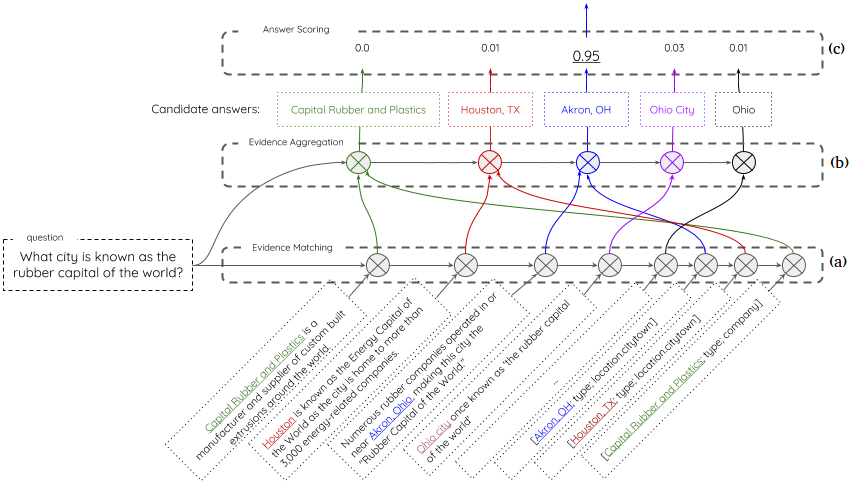
\includegraphics[width=\textwidth]{img/EviNet}
\caption{The architecture of EviNets Neural Networks for combining textual and KB evidence in factoid question answering.}
\label{figure:factoid:evinet:model}
\end{figure}

The high level architecture of \textit{EviNets} is illustrated in Figure~\ref{figure:factoid:evinet:model}.
For a given question, we extract potentially relevant information, \eg sentences from documents retrieved from text corpora using a search system.
Next, we can use an entity linking system, such as TagMe~\cite{ferragina2010tagme}, to identify entities mentioned in the extracted information, which become candidate answers.
\textit{EviNets} can further incorporate additional supporting evidence, \eg textual description of candidate answer entities, and potentially useful KB triples, such as types~\cite{Sun:2015:ODQ:2736277.2741651}.
Finally, question, answer candidates and supporting evidence are given as input to the \textit{EviNets} neural network.

\begin{figure}[t]
\centering
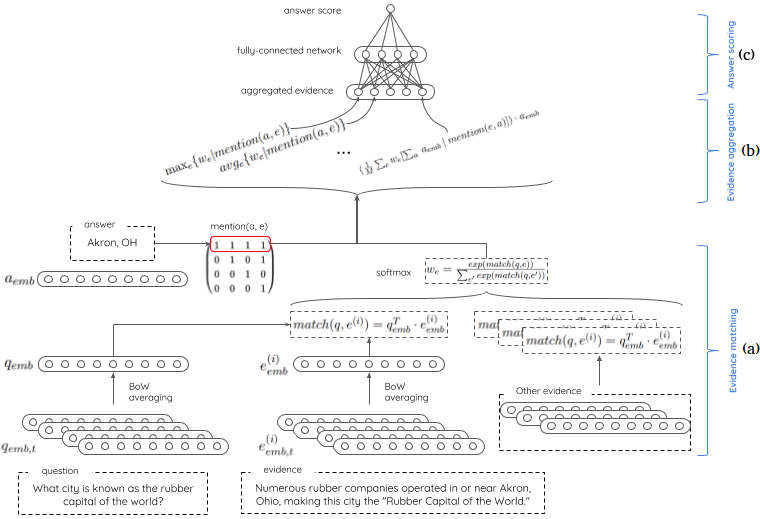
\includegraphics[width=\textwidth]{img/EviNetLayers}
\caption{Layer-wise structure of the EviNets Neural Networks framework for factoid question answering. Evidence matching (a), aggregation (b) and answer scoring (c) stages correspond to those in Figure~\ref{figure:factoid:evinet:model}.}
\label{figure:factoid:evinet:layers}
\end{figure}

Let us denote a question by $q$, and $\{q_t\in~R^{|V|}\}$, as a one-hot encoding of its tokens from a fixed vocabulary $V$.
$a_i$ is a candidate answer from the set $A$, and we will assume, that each answer is represented as a single entity.
For each question, we have a fixed set $E=E_{text} \cup E_{KB}$ of evidence statements $e^{(i)}, i=1..M$, and their tokens $e_t^{(i)}$.
A boolean function $mention:~A\times E\rightarrow\{0, 1\}$ provides the information about which answer candidates are mentioned in which evidences.
Individual tokens $q_t, a_i, e_t^{(i)}$ are translated into the embedding space using a matrix $W_{D\times~|V|}$, where $D$ is the dimension of the embeddings, \ie $q_{emb,t}~=~Wq_t$, $a_{emb,i}~=~Wa_t$ and $e^{(i)}_{emb,t}~=~We^{(i)}_t$.
In the experiments, I use the same matrix for questions, evidence, and answers.
KB entities are considered to be individual tokens, while predicates and type names are tokenized into constituent words, \ie by splitting on underscore and dot characters for Freebase predicates.
A layer-wise architecture of \textit{EviNets} is displayed on Figure~\ref{figure:factoid:evinet:layers}.
The evidence matching module ((a) on Figures~\ref{figure:factoid:evinet:model} and \ref{figure:factoid:evinet:layers}) estimates the relevance of each statement in the memory, and computes their weights using the softmax function.
The evidence aggregation module (b) uses multiple ways to compute the aggregated statistics of evidences, mentioning each answer candidate.
Finally, the answer scoring module (c) uses a fully connected network to predict a score for each answer candidate.
EviNets selects the answer with the highest score as the final response.

\subsubsection{Evidence Matching Module}

Evidence matching is responsible for estimating the relevance of each of the pieces of evidence to the question, i.e., $w_e~=~softmax(match(q, e))$.
The function \textit{match(q, e)} can be implemented using any of the recently proposed semantic similarity estimation architectures\footnote{e.g., see the ACL Wiki on Question\_Answering\_(State\_of\_the\_art).}.
One of the simplest approaches is to average question and each evidence token embeddings and score the similarity using the dot product: $q_{emb} = \frac{1}{L_q}\sum_t q_{emb,t}$ and $e^{(i)}_{emb} = \frac{1}{L_e}\sum_t e^{(i)}_{emb,t}$ and $match(q, e^{(i)}) = q^T_{emb} \cdot e^{(i)}_{emb}$.

\subsubsection{Evidence Aggregation Module}

\begin{table}[h!]
\centering
\small
\begin{tabular}{p{5.2cm}|p{7.8cm}}
Evidence Feature & Description \\
\hline
Maximum evidence score mentioning the answer & $\max_e \{w_e | mention(a, e)\}, e\in E,E_{text}~or~E_{KB}$ \\
Average evidence score mentioning the answer & $avg_e \{w_e | mention(a, e)\}, e\in E,E_{text}~or~E_{KB}$ \\
Sum of evidence scores mentioning the answer & $\sum_e \{w_e | mention(a, e)\}, e\in E,E_{text}~or~E_{KB}$ \\
Number of mentions & $\sum_e \{1 | mention(a, e)\}, e\in E_{text}$ \\
Weighted memory similarity to the question & $(\frac{1}{M}\sum_i w_e e^{(i)}_{emb})\cdot q_{emb}$\\
Weighted memory similarity to the answer~\cite{sukhbaatar2015end} & $(\frac{1}{M}\sum_i w_e e^{(i)}_{emb})\cdot a_{emb}$ or $R^T(\frac{1}{M}\sum_i w_e e^{(i)}_{emb} + q_{emb}) \cdot a_{emb}$, where $R_{D\times~D}$ is a rotation matrix \\
Weighted memory answer mentions similarity to the answer~\cite{miller2016key} & $(\frac{1}{M}\sum_e w_e [\sum_a~a_{emb}~|~mention(e, a)]) \cdot a_{emb}$ \\
\end{tabular}
\caption{Signals used in \textit{EviNets} to aggregate evidence in support for each of the answer candidates $a$.}
\label{table:factoid:evinet:aggregation}
\end{table}

After all the evidence signals have been scored, \textit{EviNets} aggregate the support for each answer candidate.
Table~\ref{table:factoid:evinet:aggregation} summarizes the aggregation features used.
With these features, \textit{EviNets} captures different aspects, \ie how well individual sentences match the question, how frequently the candidate is mentioned and how well a set of answer evidences covers the information requested in the question.

\subsubsection{Answer Scoring Module}

Finally, \textit{EviNets} uses the aggregated signals to predict the answer scores, to rank them, and to return the best candidate as the final answer to the question.
For this purpose, we use two fully-connected neural network layers with the ReLU activation function, with 32 and 8 hidden units respectively.
The model was trained end-to-end by optimizing the cross entropy loss function using the Adam algorithm~\cite{kingma2014adam}.

\subsection{Experimental Evaluation}
\label{section:factoid:evinet:eval}

\begin{table}
\small
\centering
\begin{tabular}{lp{9cm}}
Dataset & Example Questions \\
\hline
\textbf{TREC QA} & Where is the highest point in Japan? \\
1236 train & What is the coldest place on earth? \\
202 test & Who was the first U.S. president to appear on TV?\\
\hline
\textbf{WikiMovies} & what films did Ira Sachs write? \\
96185 train & what films does Claude Akins appear in? \\
10000 dev & the movie Victim starred who? \\
9952 test & what type of film is Midnight Run? \\
\hline
\textbf{Yahoo! Answers} & What is Elvis's hairstyle called? \\
1898 train & Who is this kid in Mars Attacks? \\
271 dev & who invented denim jeans? \\
542 test & who's the woman on the progressive.com commercials? \\
\end{tabular}
\caption{Statistics of the TREC QA, WikiMovies and Yahoo!~Answers factoid datasets.}
\label{table:factoid:evinet:datasets}
\end{table}


To test our framework we used TREC QA~\cite{Sun:2015:ODQ:2736277.2741651}, WikiMovies~\cite{miller2016key} benchmarks and the new Yahoo!~Answers dataset\footnote{available for research purposes at \href{url}{http://ir.mathcs.emory.edu/software-data/}} derived from factoid questions posted on the CQA website (Table~\ref{table:factoid:evinet:datasets}).
In all experiments, embeddings were initialized with 300-dimensional vectors pre-trained with Glove~\cite{pennington2014glove}.
Embeddings for multi-word entity names were obtained by averaging the word vectors of constituent words.

\subsubsection{Baselines}
\label{section:factoid:evinet:eval:baselines}

As baselines for different experiments depending on availability and specifics of a dataset we considered the following methods: 
\begin{itemize}[noitemsep,nolistsep]
\item IR-based QA systems: \textit{AskMSR}~\cite{brill2002analysis} and \textit{AskMSR+}~\cite{tsai2015web}, which select the best answer based on the frequency of entity mentions in retrieved text snippets. 
\item KBQA systems: \textit{SemPre}~\cite{BerantCFL13:sempre} and \textit{Aqqu}~\cite{bastmore:cikm:2015:aquu}, which identify possible topic entities of the question, and select the answer from the candidates in the neighborhood of these entities in a KB.
\item Hybrid system \textit{QuASE}~\cite{Sun:2015:ODQ:2736277.2741651} detects mentions of knowledge base entities in text passages, and uses the types and description information from the KB to support answer selection.
\item Hybrid system \textit{Text2KB}~\cite{Savenkov:2016:KBE:2911451.2911536}, which uses textual resources to improve different stages of the KBQA pipeline, described in Section~\ref{section:factoid:text2kb}.
\item Memory Networks: \textit{MemN2N}~\cite{sukhbaatar2015end} and \textit{KV MemN2N}~\cite{miller2016key} represent relevant information with embeddings, and summarize the memories into a single vector using the soft attention mechanism. Additionally, KV MemN2N splits memories into key-value pairs, where keys are used for matching against the question, and values are used to summarize the memories.
\end{itemize}


\subsubsection{TREC QA dataset}
\label{section:factoid:evinet:eval:trecqa}

The TREC QA dataset is composed of factoid questions, which can be answered with an entity, and were used in TREC 8-12 question answering tracks.
Similarly to~\cite{Sun:2015:ODQ:2736277.2741651} we used web search (using the Microsoft Bing Web Search API) to retrieve top 50 documents, parsed them, extracted sentences and ranked them using tf-idf similarity to the question.
To compare our results with the existing state-of-the-art, we used the same set of candidate entities as used by the QuASE model.
We note that the extracted evidence differs between the models, and we were unable to match some of the candidates to our sentences.
For text+kb experiment, just as QuASE, we used entity descriptions and types from Freebase knowledge base.

Table~\ref{table:factoid:evinet:eval:trecqa} summarizes the results.
\textit{EviNets} achieves competitive results on the dataset, beating KV MemN2N by $13\%$ in F1 score, and, unlike QuASE, does not rely on expensive feature engineering and does not require any external resources to train.

\begin{table}
\centering
\begin{tabular}{lrrr}
Method & P & R & F1 \\
\hline
SemPre & 0.157 & 0.104 & 0.125 \\
Text2KB & 0.287 & 0.287 & 0.288 \\
AskMSR+ & 0.493 & 0.490 & 0.491 \\
QuASE (text) & 0.550 & 0.550 & 0.550 \\
QuASE (text+kb) & 0.579 & \textbf{0.579} & \textbf{0.579} \\
\hline
MemN2N & 0.333 & 0.328 & 0.330 \\
KV MemN2N & 0.517 & 0.500 & 0.508 \\
EviNets (text) & 0.580 & 0.560 & 0.569 \\
EviNets (text+kb) & \textbf{0.585} & 0.564 & 0.574 \\
\end{tabular}
\caption{Precision, Recall and F1 of KB- and Text-based question answering methods on the TREC QA dataset. The improvements over the Key-Value memory networks are statistically significant at p-value $<$ 0.01.}
\label{table:factoid:evinet:eval:trecqa}
\end{table}

\subsubsection{WikiMovies dataset}
\label{section:factoid:evinet:eval:wikimovies}

The WikiMovies dataset contains questions in the movies domain along with relevant Wikipedia passages and the OMDb knowledge base.
Since KVMemN2N already achieves an almost perfect result answering the questions using the KB, we focus on using the provided movie articles from Wikipedia.
We followed the preprocessing procedures described in~\cite{miller2016key}.
Unlike TREC QA, where there are often multiple relevant supporting pieces of evidence, answers in the WikiMovies dataset usually have a single relevant sentence, which, however, mentions multiple entities.
To help the model distinguish the correct answer, and explore its abilities to encode structured and unstructured data, we generated additional \textit{entity type} triples.
For example, if an entity $e$ appears as an object of the predicate \texttt{directed\_by} in OMDb, we added the \texttt{[e, type, director]} triple.
As baselines, we used MemN2N and KV MemN2N models, and the results are presented in Table~\ref{section:factoid:evinet:eval:wikimovies}.
As we can see, with the same setup using individual sentences as evidence/memories \textit{EviNets} significantly outperforms the KV MemN2N model by $27\%$.
Moreover, the proposed approach can effectively incorporate additional entity type RDF triples, and significantly improve the performance over the text-only version.
It is important to emphasize that the best-reported results of memory networks were obtained using \textit{entity-centered windows} as memories, which requires special pre-processing and increases the number of memories.
Additionally, these models used \textit{all} of the KB entities as candidate answers, whereas \textit{EviNets} relies only on the mentioned ones, which is a more scalable scenario for open-domain question answering, where it is not realistic to score millions of candidate answers in real-time.

\begin{table}
\centering
\begin{tabular}{lr}
Method & Accuracy \\
\hline
MemN2N (wiki windows) & 0.699* \\
KV MemN2N (wiki windows) & 0.762* \\
\hline
AskMSR (entities) & 0.314 \\
KV MemN2N (wiki sent) & 0.524 \\
EviNets (wiki sent) & 0.616  \\
EviNets (wiki sent + entity types) & \textbf{0.667} \\
\end{tabular}
\caption{Accuracy of EviNets and baseline models on the WikiMovies dataset. The results marked * are obtained using a different setup, \ie they use pre-processed entity window memories, and the whole set of entities as candidates.}
\label{section:factoid:evinet:eval:wikimovies}
\end{table}

\subsubsection{New Yahoo! Answers factoid questions dataset}
\label{section:factoid:evinet:eval:yahoo}

Yahoo! recently released a dataset with search queries, which lead to clicks on factoid Yahoo!~Answers questions, identified as questions with the best answer containing less than 3 words and a Wikipedia page as the specified source of information\footnote{L27 dataset \href{url}{https://webscope.sandbox.yahoo.com}}.
This dataset contains 15K queries, which correspond to 4725 unique Yahoo!~Answers questions (Table~\ref{table:factoid:evinet:datasets}).
We took these questions, and mapped answers to KB entities using the TagMe entity linking library~\cite{ferragina2010tagme}.
We filtered out questions, for which no answer entities with a good confidence\footnote{A minimum  $\rho$ score of 0.2 from TagMe was required.} were identified, \eg date answers, and randomly split the rest into training, development and test sets, with 2711 questions in total.
Similarly to the TREC QA experiments, we extracted textual evidence using Bing Web Search API, by retrieving top 50 relevant documents, extracting the main content blocks, and splitting them into sentences.
We applied the TagMe entity linker to the extracted sentences, and considered all entities of mentions with the confidence score above the 0.2 threshold as candidate answers.
For candidate entities we also retrieved relevant KB triples, such as entity types and descriptions, which extended the original pool of evidences.

\begin{table}
\centering
\begin{tabular}{p{6cm}rrr}
Method & P & R & F1 \\
\hline
Aqqu & 0.116 & 0.117 & 0.116 \\
Text2KB & 0.170 & 0.170 & 0.170 \\
AskMSR (entities) & 0.175 & 0.319 & 0.226 \\
\hline
MemN2N & 0.072	& 0.131 & 0.092 \\
KV MemN2N & 0.126 & 0.228 & 0.162 \\
\hline
% EviNets (text) & 0.210 & 0.383 & 0.271\small{$_{+67\%}$} \\
% EviNets (text+kb) & \textbf{0.226} & \textbf{0.409} & \textbf{0.291}\small{$_{+79\%}$} \\
EviNets (text) & 0.210 & 0.383 & 0.271 \\
EviNets (text+kb) & \textbf{0.226} & \textbf{0.409} & \textbf{0.291} \\
\hline
Oracle & 0.622 & 1.0 & 0.767 \\
\end{tabular}
\caption{Precision, Recall and F1 of different methods on Yahoo! Answers factoid QA dataset. The Oracle performance assumes candidate answers are ranked perfectly and is bound by the performance of the initial retrieval step.}
\label{table:factoid:evinet:eval:yahoo}
\end{table}

Table~\ref{table:factoid:evinet:eval:yahoo} summarizes the results of \textit{EviNets} and some baseline methods on the created Yahoo!~Answers dataset.
As we can see, knowledge base data is not enough to answer most of these questions, and a state-of-the-art KBQA system Aqqu gets only 0.116 precision.
Adding textual data helps significantly, and Text2KB improves the precision to 0.17, which roughly matches the results of the AskMSR system, that ranks candidate entities by their popularity in the retrieved documents.
EviNets significantly improves over the baseline approaches, beating AskMSR by $28\%$ and KV MemN2N by almost $80\%$ in F1 score.
Using text along with KB evidence gave higher performance metrics, boosting F1 from 0.271 to 0.291.

In the above-mentioned experiments we used bag-of-words representation for questions and evidence, and a reasonable question is whether more complicated methods could achieve higher results.
Table~\ref{table:factoid:evinet:eval:yahoo_bilstm} compares bag-of-words representation with bidirectional LSTM~\cite{WangN15}.
On Yahoo!~Answers dataset BOW representation showed better performance, which is most likely due to a relatively low size of the dataset for the variety of questions present there.

\begin{table}
\centering
\begin{tabular}{lrrr}
Method & P & R & F1 \\
\hline
EviNets (text+kb): BOW & 0.226 & 0.409 & 0.291 \\
EviNets (text+kb): biLSTM & 0.196 & 0.356 & 0.252 \\
\end{tabular}
\caption{Precision, Recall and F1 of EviNets with bag-of-words and bidirectional LSTM representations of questions and evidence.}
\label{table:factoid:evinet:eval:yahoo_bilstm}
\end{table}


\subsection{Discussion}
\label{section:factoid:evinet:discussion}

\textit{EviNets}, described in this section, is a neural network for question answering, which encodes and aggregates multiple evidence signals to select answers.
Experiments on TREC QA, WikiMovies and Yahoo!~Answers datasets demonstrate that \textit{EviNets} can be trained end-to-end to use both the available textual and knowledge base information.
EviNets improves over the baselines, both in cases when there are many or just a few relevant pieces of evidence, by helping build an aggregate picture and distinguish between candidates, mentioned together in a relevant memory, as is the case for WikiMovies dataset.
The results of the experiments also demonstrate that EviNets can incorporate signals from different data sources, \eg adding KB triples helps to improve the performance over text-only setup.
As a limitation of the approach and a direction for future research, \textit{EviNets} could be extended to support dynamic evidence retrieval, which would allow retrieving additional answer candidates and evidence as needed.

% =-=-=-=-=-=-=-=-=-=-=-=-=-=-EviNets: End=-=-=-=-=-=-=-=-=-=-=-=-=-=-=-=-=-

\section{Summary}
\label{section:factoid:summary}

This Chapter introduced several approaches for combining unstructured, semi-structured and structured data sources to improve factoid question answering.
Relation extraction from question-answer pairs aims at filling some gaps in KB fact coverage.
The experiments show, that we can use distant supervision to extract factual knowledge from community question answering archives and increase the recall of the existing sentence-based relation extraction techniques.
However, extraction techniques are not perfect and suffer from both precision and recall losses.
As an alternative strategy, we can use semantic annotations of entity mentions in a text to connect knowledge base and textual data.
Such annotation allows to quickly find relevant textual resources and improve KBQA methods, as demonstrated by Text2KB model, or use both data sources together, as pieces of supporting evidence for generated answer candidates.
Diverse information can be mapped into the embedding space and aggregated together with a neural network architecture, such as \textit{EviNets}.

Factoid questions represent just a part of user information needs. Many problems require a more elaborate response, such as a sentence, list of instructions or, in general, a passage of text.
Such questions are usually referred to as non-factoid questions and they will be the focus of Chapter~\ref{chapter:non-factoid}.



% Example of the algorithm package.

% \begin{algorithm}[ht!]
% \caption[How to write a thesis]{How to write a thesis}
% \begin{algorithmic}[1]
%  \REQUIRE Some good ideas, nice figures, and some time to type it.
%  \ENSURE A nice thesis.
% \WHILE{thesis is not done}
% \STATE{keep working on it}
% \STATE{do not sleep}
% \STATE{have enough fast food at home}
% \ENDWHILE
% \FORALL{committee members}
% \STATE{take them for a beer}
% \STATE{show them the nice figures}
% \IF{they all like it}
% \STATE{\label{line:print}}{print everything and turn it in}
% \ELSE
% \REPEAT
% \STATE{\label{line:beer}}{give them another beer}
% \UNTIL{they like it}
% \ENDIF
% \ENDFOR
% \end{algorithmic}
% \end{algorithm}
